% Options for packages loaded elsewhere
\PassOptionsToPackage{unicode}{hyperref}
\PassOptionsToPackage{hyphens}{url}
\PassOptionsToPackage{dvipsnames,svgnames,x11names}{xcolor}
%
\documentclass[
]{interact}

\usepackage{amsmath,amssymb}
\usepackage{iftex}
\ifPDFTeX
  \usepackage[T1]{fontenc}
  \usepackage[utf8]{inputenc}
  \usepackage{textcomp} % provide euro and other symbols
\else % if luatex or xetex
  \usepackage{unicode-math}
  \defaultfontfeatures{Scale=MatchLowercase}
  \defaultfontfeatures[\rmfamily]{Ligatures=TeX,Scale=1}
\fi
\usepackage{lmodern}
\ifPDFTeX\else  
    % xetex/luatex font selection
\fi
% Use upquote if available, for straight quotes in verbatim environments
\IfFileExists{upquote.sty}{\usepackage{upquote}}{}
\IfFileExists{microtype.sty}{% use microtype if available
  \usepackage[]{microtype}
  \UseMicrotypeSet[protrusion]{basicmath} % disable protrusion for tt fonts
}{}
\makeatletter
\@ifundefined{KOMAClassName}{% if non-KOMA class
  \IfFileExists{parskip.sty}{%
    \usepackage{parskip}
  }{% else
    \setlength{\parindent}{0pt}
    \setlength{\parskip}{6pt plus 2pt minus 1pt}}
}{% if KOMA class
  \KOMAoptions{parskip=half}}
\makeatother
\usepackage{xcolor}
\setlength{\emergencystretch}{3em} % prevent overfull lines
\setcounter{secnumdepth}{5}
% Make \paragraph and \subparagraph free-standing
\ifx\paragraph\undefined\else
  \let\oldparagraph\paragraph
  \renewcommand{\paragraph}[1]{\oldparagraph{#1}\mbox{}}
\fi
\ifx\subparagraph\undefined\else
  \let\oldsubparagraph\subparagraph
  \renewcommand{\subparagraph}[1]{\oldsubparagraph{#1}\mbox{}}
\fi


\providecommand{\tightlist}{%
  \setlength{\itemsep}{0pt}\setlength{\parskip}{0pt}}\usepackage{longtable,booktabs,array}
\usepackage{calc} % for calculating minipage widths
% Correct order of tables after \paragraph or \subparagraph
\usepackage{etoolbox}
\makeatletter
\patchcmd\longtable{\par}{\if@noskipsec\mbox{}\fi\par}{}{}
\makeatother
% Allow footnotes in longtable head/foot
\IfFileExists{footnotehyper.sty}{\usepackage{footnotehyper}}{\usepackage{footnote}}
\makesavenoteenv{longtable}
\usepackage{graphicx}
\makeatletter
\def\maxwidth{\ifdim\Gin@nat@width>\linewidth\linewidth\else\Gin@nat@width\fi}
\def\maxheight{\ifdim\Gin@nat@height>\textheight\textheight\else\Gin@nat@height\fi}
\makeatother
% Scale images if necessary, so that they will not overflow the page
% margins by default, and it is still possible to overwrite the defaults
% using explicit options in \includegraphics[width, height, ...]{}
\setkeys{Gin}{width=\maxwidth,height=\maxheight,keepaspectratio}
% Set default figure placement to htbp
\makeatletter
\def\fps@figure{htbp}
\makeatother
% definitions for citeproc citations
\NewDocumentCommand\citeproctext{}{}
\NewDocumentCommand\citeproc{mm}{%
  \begingroup\def\citeproctext{#2}\cite{#1}\endgroup}
\makeatletter
 % allow citations to break across lines
 \let\@cite@ofmt\@firstofone
 % avoid brackets around text for \cite:
 \def\@biblabel#1{}
 \def\@cite#1#2{{#1\if@tempswa , #2\fi}}
\makeatother
\newlength{\cslhangindent}
\setlength{\cslhangindent}{1.5em}
\newlength{\csllabelwidth}
\setlength{\csllabelwidth}{3em}
\newenvironment{CSLReferences}[2] % #1 hanging-indent, #2 entry-spacing
 {\begin{list}{}{%
  \setlength{\itemindent}{0pt}
  \setlength{\leftmargin}{0pt}
  \setlength{\parsep}{0pt}
  % turn on hanging indent if param 1 is 1
  \ifodd #1
   \setlength{\leftmargin}{\cslhangindent}
   \setlength{\itemindent}{-1\cslhangindent}
  \fi
  % set entry spacing
  \setlength{\itemsep}{#2\baselineskip}}}
 {\end{list}}
\usepackage{calc}
\newcommand{\CSLBlock}[1]{\hfill\break\parbox[t]{\linewidth}{\strut\ignorespaces#1\strut}}
\newcommand{\CSLLeftMargin}[1]{\parbox[t]{\csllabelwidth}{\strut#1\strut}}
\newcommand{\CSLRightInline}[1]{\parbox[t]{\linewidth - \csllabelwidth}{\strut#1\strut}}
\newcommand{\CSLIndent}[1]{\hspace{\cslhangindent}#1}

\usepackage{booktabs}
\usepackage{caption}
\usepackage{longtable}
\usepackage{colortbl}
\usepackage{array}
\usepackage{lscape}
\newcommand{\blandscape}{\begin{landscape}}
\newcommand{\elandscape}{\end{landscape}}
\usepackage{orcidlink}
\makeatletter
\@ifpackageloaded{caption}{}{\usepackage{caption}}
\AtBeginDocument{%
\ifdefined\contentsname
  \renewcommand*\contentsname{Table of contents}
\else
  \newcommand\contentsname{Table of contents}
\fi
\ifdefined\listfigurename
  \renewcommand*\listfigurename{List of Figures}
\else
  \newcommand\listfigurename{List of Figures}
\fi
\ifdefined\listtablename
  \renewcommand*\listtablename{List of Tables}
\else
  \newcommand\listtablename{List of Tables}
\fi
\ifdefined\figurename
  \renewcommand*\figurename{Figure}
\else
  \newcommand\figurename{Figure}
\fi
\ifdefined\tablename
  \renewcommand*\tablename{Table}
\else
  \newcommand\tablename{Table}
\fi
}
\@ifpackageloaded{float}{}{\usepackage{float}}
\floatstyle{ruled}
\@ifundefined{c@chapter}{\newfloat{codelisting}{h}{lop}}{\newfloat{codelisting}{h}{lop}[chapter]}
\floatname{codelisting}{Listing}
\newcommand*\listoflistings{\listof{codelisting}{List of Listings}}
\makeatother
\makeatletter
\makeatother
\makeatletter
\@ifpackageloaded{caption}{}{\usepackage{caption}}
\@ifpackageloaded{subcaption}{}{\usepackage{subcaption}}
\makeatother
\ifLuaTeX
  \usepackage{selnolig}  % disable illegal ligatures
\fi
\usepackage{bookmark}

\IfFileExists{xurl.sty}{\usepackage{xurl}}{} % add URL line breaks if available
\urlstyle{same} % disable monospaced font for URLs
\hypersetup{
  pdftitle={Frequency attenuation effects in masked repetition priming: A large scale online lexical decision study},
  pdfauthor={Roberto Petrosino; Diogo Almeida},
  pdfkeywords={masked repetition priming, frequency attenuation
effect, online browser-based experiment, power analysis},
  colorlinks=true,
  linkcolor={blue},
  filecolor={Maroon},
  citecolor={Blue},
  urlcolor={Blue},
  pdfcreator={LaTeX via pandoc}}

\title{Frequency attenuation effects in masked repetition priming: A
large scale online lexical decision study}
\author{Roberto
Petrosino$\textsuperscript{1}$~\orcidlink{0000-0002-8502-3070}, Diogo
Almeida$\textsuperscript{1}$~\orcidlink{0000-0003-4674-8092}}

\thanks{CONTACT: Roberto
Petrosino. Email: \href{mailto:roberto.petrosino@nyu.edu}{\nolinkurl{roberto.petrosino@nyu.edu}}. Diogo
Almeida. Email: \href{mailto:diogo@nyu.edu}{\nolinkurl{diogo@nyu.edu}}. }
\begin{document}
\captionsetup{labelsep=space}
\maketitle
\textsuperscript{1} Psychology Program, Division of Science, New York
University Abu Dhabi, Abu Dhabi, United Arab Emirates
\begin{abstract}
This study addresses the controversy surrounding the sensitivity of
masked repetition priming to word frequency, a topic less contentious in
unmasked priming. While unmasked priming exhibits a frequency
attenuation effect, wherein high frequency words yield smaller
repetition effects, this phenomenon has been inconsistently reported in
masked priming. We conducted two large online experiments with
rigorously validated frequency databases to reconcile past
discrepancies. The first experiment confirmed masked repetition
priming's viability in web browser-based settings. The pre-registered
second study, designed for high statistical power, successfully
identified a significant 9-ms frequency attenuation effect under masked
priming conditions. This result indicates that the repetition effect in
masked priming is less qualitatively distinct from unmasked priming than
previously assumed, a finding with important practical and theoretical
consequences. Moreover, our research underscores the usefulness of
online masked priming experiments for detecting subtle effects that may
elude traditional lab-based investigations.
\end{abstract}
\begin{keywords}
\def\sep{;\ }
masked repetition priming\sep frequency attenuation effect\sep online
browser-based experiment\sep 
power analysis
\end{keywords}

\section{Introduction}\label{sec-intro}

The masked priming technique has been an invaluable tool in visual word
recognition research. It has allowed researchers to study the conditions
under which orthographic, phonological, morphological, and semantic
information impact access to visual word forms while mitigating
strategic effects and minimizing the influence of controlled processes
(Forster 1998). First introduced in its traditional form by Forster and
Davis (1984; see also Evett and Humphreys 1981), this technique involves
a forward mask (i.e., usually a string of hashes, \#\#\#\#\#), followed
by a prime string presented for very short time (\(SOA < 60\)
ms),\footnote{\emph{SOA: Stimulus Onset Asynchrony}, i.e.~the time
  between the start of one stimulus (in our case, the prime stimulus)
  and the start of another stimulus (the target stimulus). In the
  standard repetition priming design, no backward mask occurs between
  the prime and the target, and therefore SOA equals the duration of
  prime presentation.} and a target string presented immediately after.
Because the prime presentation is so brief and masked by preceding and
subsequent stimuli, most participants report not being aware that a
prime string had been presented, and can at most report a screen flicker
just before the target presentation (Forster, Mohan, and Hector 2003).

Among possible manipulations of prime-target relatedness, masked
repetition priming (in which the same word is presented as both the
prime and target within the same trial: e.g., \emph{love-LOVE}) has been
well studied, because its response seems to be qualitatively different
from the unmasked counterpart (\(SOA > 60 ms\)): while high-frequency
words benefit less from repetition than low-frequency words in the
unmasked design (\emph{frequency attenuation effect}, henceforth FAE;
Scarborough, Cortese, and Scarborough 1977), this does not seem to be
the case when the prime is masked (Forster and Davis 1984; Forster et
al. 1987; Segui and Grainger 1990; Sereno 1991; Forster and Davis 1991;
Rajaram and Neely 1992; Bodner and Masson 1997; Forster, Mohan, and
Hector 2003; Nievas 2010).

This asymmetry in sensitivity to lexical frequency between the masked
and unmasked repetition priming responses has been important in
distinguishing among different models of priming in visual word
recognition. More specifically, \emph{interactive activation models}
(McClelland and Rumelhart 1981; Grainger and Jacobs 1996; Coltheart et
al. 2001) conceive of priming as a ``head start'' in processing due to
the pre-activation of the target word due to the presentation of the
prime. According to this type of model, priming is ultimately due to
this single mechanism, and therefore it is difficult to reconcile
interactive activation models with the qualitatively different profiles
for repetition priming in masked and unmasked conditions.

Similarly, episodic models (e.g., Jacoby and Dallas 1981; Jacoby 1983)
posit a different single mechanism for priming effects, that is, the
activation/retrieval of the episodic memory trace of the encounter with
the prime word. These models therefore encounter the same type of
difficulty in accounting for qualitatively different patterns of
repetition priming effects in masked and unmasked conditions. A similar
type of model, called the \emph{memory recruitment model} makes very
similar predictions to the episodic memory models, positing a
non-lexical source for priming effects (Bodner and Masson 1997; Masson
and Bodner 2003; Bodner and Masson 2014). Repetition priming effects
under this view stem from the exploitation, strategically or
automatically, of a memory resource created by the encounter with the
prime word. The frequency attenuation effect, under episodic and memory
recruitment models alike, is predicted on the basis that low frequency
primes, being more distinctive stimuli, create a more potent and
effective memory resource compared to high frequency primes.

Alternatively, other models with a more fine-grained view of the lexical
access process seem to sidestep the problem posed by the qualitatively
different repetition priming profiles observed in masked and unmasked
conditions. One such model is the \emph{entry-opening model} (also known
as the bin model; Forster and Davis 1984). According to this model, when
the visual stimulus is presented, lexical entries are assigned to
specific bins based on orthographic similarity. In the first stage (fast
search stage), a fast, frequency-ordered search goes through the entries
within a given bin, and compares each one with the the input stimulus,
thus assigning to each entry a goodness-of-fit score. This comparison is
fast and crude, and sorts entries into (a) perfect (i.e., no difference
is detected between the input and the entry), (b) close (i.e., small
differences are detected), and (c) irrelevant matches (i.e., substantial
difference are detected). Any entry of type (a) or (b) is opened, so
that the entry can be further analyzed and compared to the input in the
subsequent verification stage. In the masked environment, the entry of
the prime word is opened at the fast search stage, but its short
presentation duration prevents it from reaching the evaluation stage,
but the entry is nonetheless left open. Upon the presentation of the
target, the access procedure will follow its two stage course, with a
frequency-sensitive fast search and a subsequent entry opening for
evaluation/verification. In this view, the fast search for the target
word proceeds normally, but the evaluation/verification procedure starts
and ends sooner than it otherwise would, because the target entry has
already been left open after the brief processing of the prime. Thus,
the \emph{entry-opening model} explains the masked repetition priming as
the benefit from having the entry of the target word already open when
it is going to be evaluated in the second stage of recognition.
Crucially, this occurs \emph{after} the target word is initially
accessed, which happens in order of frequency. Put differently,
according to the \emph{entry-opening model}, masked repetition priming
occurs because of the time savings from not having to open the entry,
which is a frequency-insensitive process (every entry takes the same
time to be opened), but \emph{after} the frequency-sensitive first
access stage. As a consequence, \emph{entry-opening model} predicts a
frequency-insensitive masked repetition priming effect, which is what
has been traditionally reported in the literature (see
Table~\ref{tbl-litReview}). In addition, it also (correctly) predicts
that pseudowords should not benefit from masked repetition priming, as
they have no entries in the mental lexicon to be left open after the
brief processing of the prime.

However, as Table~\ref{tbl-litReview} shows, there are nonetheless a few
studies that do report significant FAEs in masked repetition priming
(Bodner and Masson 2001; Kinoshita 2006; Norris and Kinoshita 2008).
Bodner and Masson (2001) report that when stimuli are presented in
alternating case (e.g., \emph{pHoNe}), this increases the lexical
decision difficulty and therefore creates an extra incentive to draw on
the memory resource created by the brief processing of the prime. Under
such conditions, they were able to observe a statistically significant
FAE. In the same vein, Kinoshita (2006) noticed that in earlier studies
the low frequency words often had very high error rates, and suggested
that perhaps many participants did not know them. If participants
treated a substantial number of low frequency words as nonwords, and
nonwords do not exhibit repetition priming under masked conditions, it
could artificially depress the repetition priming effect. In two
separate experiments, Kinoshita (2006) showed that larger repetition
priming effects for low frequency words were only obtained when the low
frequency words were vetted to make sure the participants knew them
prior to the experiment. Following up on Kinoshita (2006), Norris and
Kinoshita (2008) were also able to find an interaction between lexical
frequency and repetition in masked repetition priming.

Finally, as Table~\ref{tbl-litReview} shows, it is noteworthy that 15
out of 18 previous studies showed numerically larger masked priming
effects for low frequency words as opposed to high frequency words,
irrespective of statistical significance. Similarly, the average
repetition effect for low frequency words in the studies reviewed in
Table~\ref{tbl-litReview} is 13 ms larger when compared to that of high
frequency words. These results are not in line with the predictions
dictated by the \emph{entry opening model}, and seem to align better
with the predictions made by \emph{interactive activation models} and
\emph{memory recruitment} models.

\blandscape

\setlength{\LTpost}{0mm}

\begin{longtable}{l|lrlrrrrll}

\caption{\label{tbl-litReview}Summary of the masked repetition priming
effects as a function of word frequency reported in the literature. The
power range estimates were calculated by simulating 10,000 datasets with
the corresponding sample size (N) and FAE = 15 ms and 30 ms.}

\tabularnewline

\toprule
\multicolumn{1}{l}{} &  &  &  & \multicolumn{2}{c}{MOP (ms)} & \multicolumn{2}{c}{FAE (ms)} & \multicolumn{2}{c}{Power range [min max]} \\ 
\cmidrule(lr){5-6} \cmidrule(lr){7-8} \cmidrule(lr){9-10}
\multicolumn{1}{l}{Study} & Language & N & SOA & HF & LF & ES & \emph{p}\textless{}.05? & FAE=15ms & FAE=30ms \\ 
\midrule\addlinespace[2.5pt]
Forster, Davis, Schoknecht, \& Carter (1987), exp. 1 & English & 16 & 60 & 61 & 66 & 5 &   & [0.02 0.24] & [0.04 0.84] \\ 
Norris, Kinoshita, Hall, \& Henson (2018) & English & 16 & 50 & 38 & 51 & 13 &   & [0.02 0.24] & [0.04 0.84] \\ 
Sereno (1991), exp. 1 & English & 20 & 60 & 40 & 64 & 24 &   & [0.02 0.33] & [0.04 0.92] \\ 
Forster \& Davis (1991), exp. 5 & English & 24 & 60 & 54 & 72 & 18 &   & [0.02 0.4] & [0.05 0.96] \\ 
Bodner \& Masson (1997), exp. 1 & English & 24 & 60 & 29 & 45 & 16 &   & [0.02 0.4] & [0.05 0.96] \\ 
Bodner \& Masson (1997), exp. 3 & English & 24 & 60 & 36 & 50 & 14 &   & [0.02 0.4] & [0.05 0.96] \\ 
Forster, Mohan, \& Hector (2003), exp. 1 & English & 24 & 60 & 63 & 60 & -3 &   & [0.02 0.4] & [0.05 0.96] \\ 
Kinoshita (2006), exp. 1 & English & 24 & 53 & 32 & 38 & 6 &   & [0.02 0.4] & [0.05 0.96] \\ 
Kinoshita (2006), exp. 2 & English & 24 & 53 & 29 & 59 & 30 & * & [0.02 0.4] & [0.05 0.96] \\ 
Norris \& Kinoshita (2008), exp. 1 & English & 24 & 53 & 35 & 66 & 31 & * & [0.02 0.4] & [0.05 0.96] \\ 
Forster, Davis, Schoknecht, \& Carter (1987), exp. 4 & English & 27 & 60 & 34 & 25 & -9 &   & [0.03 0.46] & [0.05 0.98] \\ 
Forster \& Davis (1984), exp. 1 & English & 28 & 60 & 45 & 38 & -7 &   & [0.03 0.48] & [0.06 0.98] \\ 
Nievas (2010), exp. 1b & Spanish & 30 & 50 & 44 & 65 & 21 & * & [0.03 0.52] & [0.06 0.99] \\ 
Nievas (2010), exp. 2a & Spanish & 30 & 50 or 33\textsuperscript{\textit{1}} & 51 & 58 & 7 &   & [0.03 0.52] & [0.06 0.99] \\ 
Segui \& Grainger (1990), exp. 4 & French & 36 & 60 & 42 & 45 & 3 &   & [0.03 0.63] & [0.07 1] \\ 
Bodner \& Masson (2001), exps. 2A, 2B, 3, \& 6 (average)\textsuperscript{\textit{2}} & English & 40 & 60 & 37 & 69 & 32 & * & [0.03 0.68] & [0.08 1] \\ 
Rajaram \& Neely (1992), exp. 1 & English & 48 & 50 & 30 & 37 & 7 &   & [0.04 0.76] & [0.09 1] \\ 
Rajaram \& Neely (1992), exp. 2 & English & 48 & 50 & 45 & 78 & 33 &   & [0.04 0.76] & [0.09 1] \\ 
\midrule 
\midrule 
Mean &   &   &   & 41 & 55 & 13 &   &   &   \\ 
SD &   &   &   & 10 & 14 & 13 &   &   &   \\ 
Correlation &   &   &   &   &   & 0.46 &   &   &   \\ 
\bottomrule

\end{longtable}

\begin{minipage}{\linewidth}
\textsuperscript{\textit{1}}SOA for each subject determined by pre-test\\
\textsuperscript{\textit{2}}Reported in Masson \& Bodner (2003)\\
\end{minipage}

\elandscape

\section{The present study}\label{sec-study}

It is somewhat surprising that the status of the FAE in masked priming
remains largely unresolved in the literature, given its substantial
magnitude (especially considering that the difference between two
conditions seems to be statistically significant: \emph{M\_FAE} = 13,
CI\_95\% = {[}7, 20{]}), \emph{t}(17) = 4.24, \(p=.0005\)), and its
theoretical significance in elucidating the underlying cognitive
processes of masked priming.

One possible interpretation of the conflicting past findings revolves
around the fact that only 4 out of 18 studies demonstrate a
statistically significant FAE in masked repetition priming. Notably,
this number potentially diminishes further when considering that, among
these four studies, the FAE is detected only through the pooling of data
across multiple studies employing a unique alternating-case stimulus
presentation (Bodner and Masson 2001; Masson and Bodner 2003). This line
of reasoning suggests a qualitatively distinct profile between masked
and unmasked repetition priming, with the FAE more firmly established in
the latter.

Conversely, one could argue that 15 out of 18 studies exhibit
numerically larger repetition effect sizes for low-frequency words
compared to high-frequency words ---- a pattern that is challenging to
reconcile with a genuine absence of interaction between frequency and
masked repetition. Additionally, the average FAE across all studies
stands at 13 ms, a modest yet non-negligible (and statistically
significant) effect size. These considerations suggest that a genuine
FAE may exist in masked priming but might be smaller than the thresholds
detectable by most previous experiments.

Compounding this complexity, another potential contributor to past
discrepancies is the reliance on the dated Kucera and Francis (1967)
word frequency database, which 15 out of 18 studies have depended on.
This poses a potential problem, as this frequency database has
consistently demonstrated inferior predictive performance, particularly
with low-frequency words, compared to more contemporary databases
(Burgess and Livesay 1998; Zevin and Seidenberg 2002; Balota et al.
2004; Brysbaert and New 2009; Yap and Balota 2009; Brysbaert and Cortese
2011; Gimenes and New 2016; Herdağdelen and Marelli 2017; Brysbaert,
Mandera, and Keuleers 2018). Both of these issues are addressed in the
subsequent sections.

\subsection{Issues with frequency databases}\label{sec-study-freq}

Due to the well-documented concerns over the reliability of the Kučera
and Francis (1967) frequency database for psycholinguistic experiments
(Burgess and Livesay 1998; Zevin and Seidenberg 2002; Balota et al.
2004; Brysbaert and New 2009; Yap and Balota 2009; Brysbaert and Cortese
2011; Gimenes and New 2016; Herdağdelen and Marelli 2017; Brysbaert,
Mandera, and Keuleers 2018), our studies exclusively sourced materials
from the HAL (Lund and Burgess 1996) and SUBTLEX\({US}\) (Brysbaert and
New 2009) databases, which reflect more recent linguistic usage and
offer better validation in behavioral experiments (e.g., Balota et al.
2004; Brysbaert and New 2009; Yap and Balota 2009; Brysbaert and Cortese
2011; Gimenes and New 2016; Herdağdelen and Marelli 2017). While these
databases outperform Kučera and Francis (1967) in predicting
psycholinguistic task outcomes, it is important to note potential
discrepancies in individual frequency counts, particularly in the low
and mid-frequency ranges. This variation, attributable to the primary
genre of their sources (USENET groups for HAL and movie subtitles for
SUBTLEX\(_{US}\)),\footnote{A separate, though relevant issue which
  cannot be addressed here is to how to mitigate the discrepancies
  across the databases available, but see Yap and Balota (2009), and
  Brysbaert and Cortese (2011) for proposals about combining the
  frequency counts from different corpora.\label{fn-databases}} may have
minimal impact on megastudies with large word samples (e.g., Balota et
al. 2004; Brysbaert and New 2009; Yap and Balota 2009; Brysbaert and
Cortese 2011; Gimenes and New 2016; Herdağdelen and Marelli 2017).
However, corpus-specific frequency skew can become significant when
dealing with smaller samples of words in studies such as masked priming.
Table~\ref{tbl-exFreqSkew} illustrates the potential discrepancy in
considering words as high or low frequency based on the different
aforementioned databases.

\begin{longtable}{lrrr}

\caption{\label{tbl-exFreqSkew}Example of frequency count imbalances (in
occurrences per million) across the frequency norms of Kucera \& Francis
(KF), HAL and SUBTLEX\textsubscript{US} for 4 to 6 letter words.}

\tabularnewline

\toprule
Word & KF & HAL & SUBTLEX\textsubscript{US} \\ 
\midrule\addlinespace[2.5pt]
\multicolumn{4}{l}{\emph{Skew in KF}} \\ 
\midrule\addlinespace[2.5pt]
negro & $104$ & $3$ & $5$ \\ 
poet & $99$ & $9$ & $9$ \\ 
mercer & $71$ & $4$ & $2$ \\ 
swung & $48$ & $3$ & $2$ \\ 
mantle & $48$ & $8$ & $2$ \\ 
\midrule\addlinespace[2.5pt]
\multicolumn{4}{l}{\emph{Skew in HAL}} \\ 
\midrule\addlinespace[2.5pt]
web & $6$ & $351$ & $9$ \\ 
user & $4$ & $297$ & $2$ \\ 
mint & $7$ & $211$ & $5$ \\ 
format & $9$ & $198$ & $1$ \\ 
warp & $4$ & $125$ & $5$ \\ 
\midrule\addlinespace[2.5pt]
\multicolumn{4}{l}{\emph{Skew in SUBTLEX\textsubscript{US}}} \\ 
\midrule\addlinespace[2.5pt]
daddy & $4$ & $16$ & $185$ \\ 
bitch & $6$ & $24$ & $169$ \\ 
cute & $5$ & $28$ & $88$ \\ 
pardon & $8$ & $12$ & $65$ \\ 
steal & $5$ & $28$ & $53$ \\ 
\bottomrule

\end{longtable}

\subsection{Issues with statistical power}\label{sec-study-power}

The inconsistency of past findings regarding the FAE in masked priming
has been linked to a potential lack of statistical power in previous
research (Bodner and Masson 1997, 2001; Masson and Bodner 2003). This is
a plausible concern, as interactions like the FAE often require larger
sample sizes for statistical detection (Potvin and Schutz 2000;
Brysbaert and Stevens 2018) compared to main effects. We outline below
three ways in which neglecting statistical power might frustrate our
understanding of FAE in masked repetition priming.

First, our literature review revealed crucial gaps in reporting relevant
statistical information, obstructing the assessment of the statistical
power attained by past experiments. The inconsistent reporting of each
conditions' standard deviations (only 7 out of 18 studies) and the
complete lack of reporting of the correlation structure between
conditions complicates power assessments. Researchers are thus forced to
explore a range of plausible values for standard deviations and
correlation structures on their own.

Table~\ref{tbl-litReview} details our attempt to conduct power
simulations for two hypothesized frequency attenuation effect sizes: 15
ms, close to the averaged FAE of 13 ms, and 30 ms, close to the only
four observed statistically significant FAE. Standard deviations
(ranging between 60 ms and 180 ms, in 10 ms increments) and correlation
between conditions (uniformly set to range between 0.6 and 0.9, with 0.1
unit increments) were simulated for each study's sample size, with
10,000 replications for each simulation. These range of values were
derived from our literature review and previous in lab and online
experiments (Petrosino 2020; Petrosino, Sprouse, and Almeida 2023). For
each simulated dataset, a paired \emph{t}-test was performed comparing
the repetition effect for high frequency words and low frequency words.
This calculation is mathematically identical to the interaction term in
a 2x2 factorial within-subjects design, but it is less computationally
expensive to perform in large scale simulations. Power to detect this
interaction was then calculated as the proportion of significant tests
obtained across replications. All else being equal, standard deviations
and correlations between conditions have opposite effects on statistical
power: increases in standard deviations lead to less power, while
increases in correlation between conditions lead to more power.

The results reported in Table~\ref{tbl-litReview} reveal a wide range of
possible statistical power attained by previous studies, depending
solely on the combination of plausible standard deviation and
correlation across conditions. For instance, the study with the smallest
sample size (Forster et al. 1987, \(N=16\)) had a 2\% to 24\% chance of
detecting a 15 ms frequency attenuation effect and a 4\% to 84\% chance
for a 30 ms effect. Similarly, the study with the largest sample size
(Rajaram and Neely 1992, \(N=48\)) exhibited a range of 4\% to 76\% for
a 15 ms frequency attenuation effect and 9\% to 100\% for a 30 ms
effect. As a consequence of the limited reporting of relevant
statistical information in past studies, it is nearly impossible to
determine if any of them were adequately powered to detect the effect of
interest.

A second concern arising from the ambiguity surrounding statistical
power in the literature is the potential impact of a prevalence of
low-powered experiments on the scientific record. An excess of such
experiments increases the risk of observed statistically significant
effects being spurious (Button et al. 2013). As highlighted in
Table~\ref{tbl-litReview}, only 4 out of 18 studies demonstrate a
statistically significant FAE. The absence of clarity regarding the
statistical power of previous research poses challenges in assessing the
likelihood of these significant findings being spurious.

Finally, it is widely acknowledged that experiments with approximately
50\% power are akin to a coin toss in their ability to detect a true
effect (Cohen 1992). A less-appreciated fact is that, in the presence of
even lower power (\textless25\%), statistically significant results can
substantially overestimate the effect size -- a type-M error (Gelman and
Carlin 2014). When power drops to levels below 10\%, a statistically
significant result may occur even when the observed effect goes in the
opposite direction of the true effect -- a type-S error (Gelman and
Carlin 2014). Our power simulations for within-subjects data revealed a
similar relationship between statistical power, type-M, and type-S
errors in line with the observations detailed by Gelman and Carlin
(2014) for the independent samples \(t\)-test. For instance, at 10\%
power (a possibility for virtually all previous studies, as indicated in
Table~\ref{tbl-litReview}), a statistically significant result could
indicate an overestimation of the magnitude of the frequency attenuation
effect by a factor between 2 and 5, with a 5\% chance of incorrectly
determining the direction of the effect.

\begin{figure}[H]

\centering{

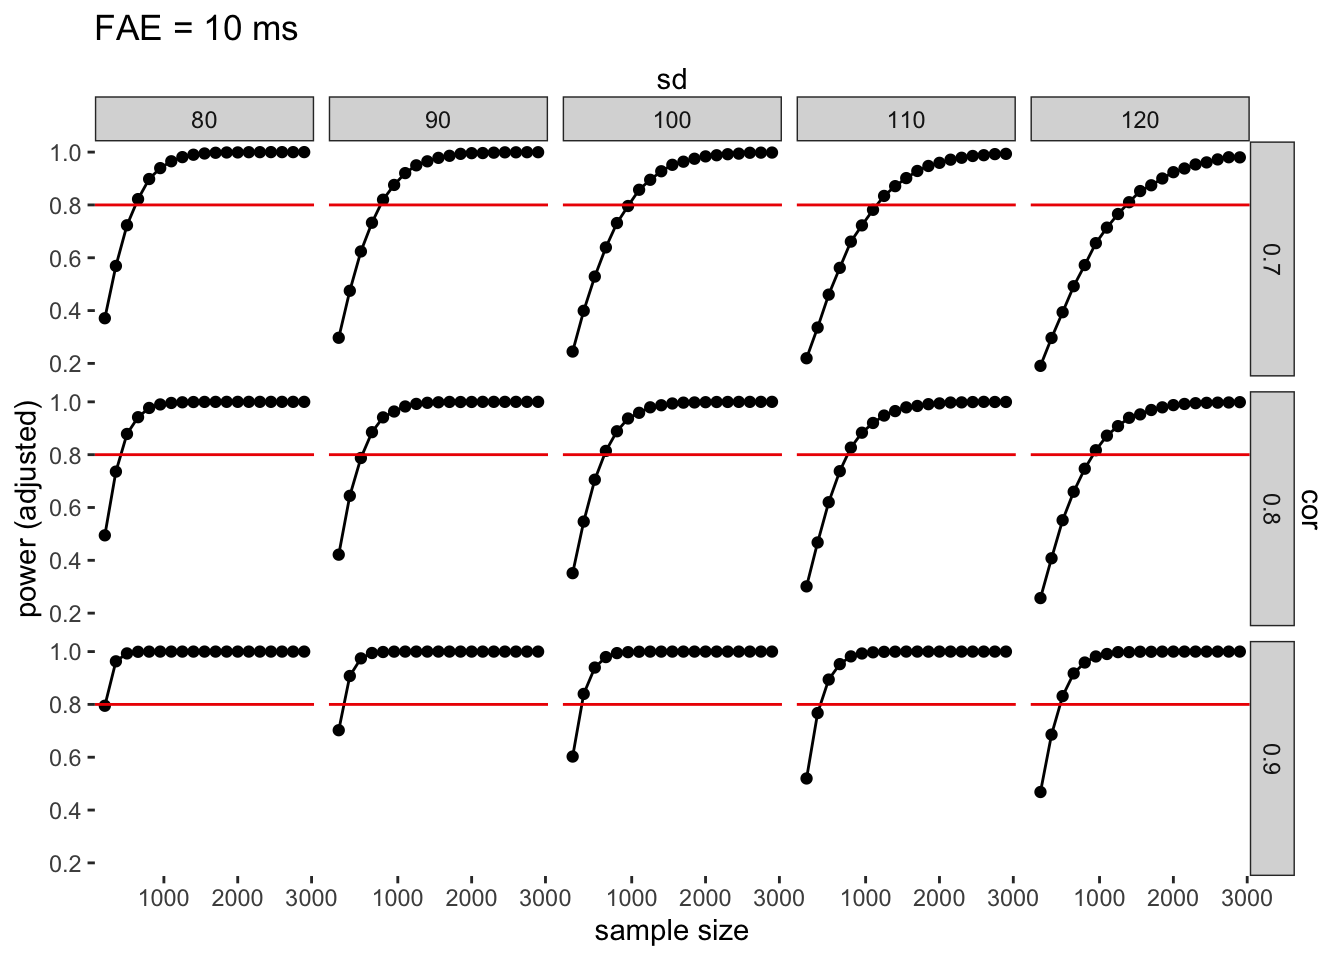
\includegraphics{index_files/figure-latex/notebooks-intro_lit-review_power-analysis-fig-power-output-1.png}

}

\caption{\label{fig-power}Power simulations for a FAE = 10 ms, for all
combinations of standard deviation (sd), correlation (cor), and sample
size. The red line identifies the threshold of 80\% power.}

\end{figure}%

The two studies reported here were designed to mitigate these two
confounding issues: the overreliance on the Kučera and Francis (1967)
frequency data as well as a potential lack of statistical power observed
in previous research. As a large increase in statistical power requires
a large sample size, Experiment 1 aimed to assess the suitability of
using \emph{Labvanced} (Finger et al. 2017), an online platform for
running web browser-based experiments, for running masked priming
studies online.

\section{Experiment 1}\label{sec-exp1}

As evident in Table~\ref{tbl-litReview}, conducting a properly powered
experiment for a FAE close to the averaged value calculated from
previous studies will require sample sizes that would be impractical to
pursue in standard university research settings, typically quiet lab
rooms with limited research computers. In response to this challenge,
our study was exclusively conducted online, leveraging the growing trend
in online behavioral research facilitated by HTML5 capabilities and the
availability of advanced web software such as \emph{jsPsych} (Leeuw
2014), \emph{PsychoJS} (the JavaScript counterpart of \emph{PsychoPy},
Peirce et al. (2019)), \emph{Gorilla} (Anwyl-Irvine et al. 2020), and
\emph{Labvanced} (Finger et al. 2017).

Notably, two recent studies have already demonstrated the viability of
conducting masked priming experiments online, employing different
software tools: Angele et al. (2023) with \emph{PsychoJS}, and Cayado,
Wray, and Stockall (2023) with \emph{Gorilla}. In our study, we opted
for \emph{Labvanced} (Finger et al. 2017). This choice was motivated by
our university's recent acquisition of a group license for
\emph{Labvanced}, itself motivated by its user-friendly GUI-based web
app nature. Similar to \emph{Gorilla}, \emph{Labvanced} eliminates local
installation issues, ensuring cross-platform consistency and simplifying
experimental design without necessitating proficiency in additional
programming languages.

\subsection{Methods}\label{sec-exp1-methods}

\subsubsection{Materials}\label{sec-exp1-methods-materials}

Two hundred five-letter English words were selected from the English
Lexicon Project (ELP; Balota et al. 2007), in which 100 words were
selected from an upper and a lower frequency range,
respectively.\footnote{The experiment also included an even lower
  frequency condition (range: {[}3.0 5.01{]}; mean: 4.39, SD: 0.50),
  thus summing up to six hundred trials being presented in the
  experiment. However, the average error rate for this condition was
  44\% and 33 (out of the 50) target words used in the same condition
  had a error rate higher than 30\%. This suggested that they might have
  not known these words at all (see Kinoshita (2006)). For this reason,
  this condition was completely removed from analysis and will not be
  mentioned in the rest of this article.} It was not possible to
identify two frequency ranges that were well separated from one another
for both the HAL (Lund and Burgess 1996) and the SUBTLEX\(_{US}\)
(Brysbaert and New 2009) frequency databases. As
Table~\ref{tbl-words_exp1} shows, we managed to do this only for the
former, whereas some overlap was present in the latter, as expected
given the different source of the two databases (see above, and fn.
\ref{fn-databases}). The two word subsets corresponded to the two word
frequency conditions being tested: the high-frequency, and low-frequency
conditions. In each condition, fifty words were randomly chosen to be
presented as targets and related primes (for the related prime type
condition), and the remaining fifty were presented as unrelated primes
(for the unrelated prime type condition).

\begin{longtable}{crrrrrrrrr}

\caption{\label{tbl-words_exp1}Experiment 1. Descriptive statistics of
the word item used. For both frequency databases, the word frequencies
were converted to per-million count to ensure cross-comparison.}

\tabularnewline

\toprule
 &  & \multicolumn{4}{c}{\textbf{HAL}} & \multicolumn{4}{c}{\textbf{SUBTLEX\textsubscript{US}}} \\ 
\cmidrule(lr){3-6} \cmidrule(lr){7-10}
frequency & N & min & max & mean & SD & min & max & mean & SD \\ 
\midrule\addlinespace[2.5pt]
high & 100 & 169 & 1212 & 482 & 292 & 2.00 & 1168 & 129 & 201 \\ 
low & 100 & 3 & 23 & 9 & 5 & 0.12 & 13 & 3 & 3 \\ 
\bottomrule

\end{longtable}

Two-hundred five-letter phonotactically legal nonwords were randomly
selected from the ELP database as well. Half of them were randomly
selected to be presented as targets; the other half was instead used as
unrelated nonword primes.

\subsubsection{Participants}\label{sec-exp1-methods-participants}

Three hundred participants (145 females; age mean: 38.48; age sd: 12.44)
were recruited on Prolific (\url{https://www.prolific.com}). Several
criteria were selected to ensure recruitment of native speakers of U.S.
English. Participants needed to be born in the Unites States of America,
speak English as their first and only language, and have no
language-related disorder. We encouraged participants to avoid any sort
of distraction throughout the experiment, and to close any program that
may be running in the background, as a way to boost performance of the
stimulus presentation in the web browser as much as possible. Because
the experiment was run online, participants could not be monitored in
any way during data collection. Finally, to further reduce variability
across participants' devices, we restricted the experiment to be run on
Google Chrome only, which is the most used browser worldwide
(\url{https://www.w3counter.com/globalstats.php}), and reportedly
performs better than any other across operating systems (likely thanks
to the Blink engine; see Lukács and Gartus 2023).

\subsubsection{Procedure}\label{sec-exp1-methods-proc}

Each recruited participant was assigned one of two word lists, which
differed only in the relatedness of the prime with respect to the
target; otherwise, the two lists presented the same set of target words
and nonwords (300 items in total). In one list, the three conditions
(high-frequency, low-frequency word conditions, and the non-word
condition) had 25 target items being preceded by themselves (the
\emph{related} condition) and the remaining 25 target items being
preceded by one of the unrelated primes belonging to the same frequency
bin (the \emph{unrelated} condition). In the other list, these
assignments were reversed. The order of stimulus presentation was
randomized for each participant.

After being recruited, participants were asked to click on a link which
redirected them to Labvanced. During the experiment, they were asked to
perform a lexical decision task by pressing either the `J' (for word) or
`F' (for non-word) keys on their keyboard. Each trial consisted of three
different stimuli appearing at the center of the screen: a series of
hashes (\#\#\#\#\#) presented for 500 ms, followed by a prime word
presented for 33 ms, and finally the target word; the target word
disappeared from the screen as soon as a decision was made. The
motivation for the choice of a very short prime duration (as compared to
the literature, in which it is usually between 50 and 60 ms; see
Table~\ref{tbl-litReview}) is threefold. First, previous pilot
experiments on \emph{Labvanced} showed that, due to the inherent
difficulties in presenting stimuli for very short set durations on the
browser, a longer duration would increase the number of trials in which
the prime duration would rise above the subliminal threshold (usually
set at 60 ms) due to timing inaccuracies and missing screen refreshes,
which could trigger the adoption of experiment-wide strategies in the
task, and ultimately contaminate the masked priming response. Second,
Angele et al. (2023) and Cayado, Wray, and Stockall (2023) have
demonstrated that a 33 ms priming duration does elicit repetition
priming effects in online experiments. Finally, setting such a short
prime duration prevents virtually everyone from consciously perceiving
the prime word Nievas (2010), and thus presents a less contaminated
estimate of early automatic processes in word recognition.

Participants were given 5 breaks throughout the experiment. When the
experiment was over, the participants were then redirected to Prolific
in order to validate their submission. The median time to finish the
experiment was 11 minutes and 27 seconds. Each participant was paid with
a standard rate of GBP 9/hour.

\subsection{Data analysis}\label{sec-exp1-analysis}

Analysis scripts and an abridged version of the data collected can be
found on online (\url{https://osf.io/ej8dh}). We performed three
different steps of analyses (in sequential order), with the goal of only
keeping data that pass a set of stringent including criteria (77,359
observations in total). After removing participants and items with high
error rates, we implemented a novel pre-processing step looking at the
distribution of the actual durations of prime stimuli of each trial and
for each subject. This was necessary to understand the performance
capabilities of experiments set up by \emph{Labvanced}, and how accurate
they are in keeping the prime duration constant. Finally, we removed RT
outliers.

\subsubsection{Step 1: subject and item
performance}\label{sec-exp1-analysis-performance}

Item and subject error rates were calculated, with a cutoff of 30\%.
Only 3 low-frequency words (\emph{carte, parse, posit}), 5 non-words
(**), and 8 participants were removed, with 291 participants remaining.

\subsubsection{Step 2: prime
durations}\label{sec-exp1-analysis-primeTime}

During the experiment, the duration of presentation of the prime word
was recorded for every trial. Both the mean (mean = 37.88 ms) and the
median (median = 35 ms) of the actual prime durations were slightly
larger than the intended prime duration (33 ms). This distribution
suggests that, while overall the visual presentation was kept in most
trials at the intended duration, it was not 100\% as precise and
accurate as dedicated presentation software installed on lab computers.
This was expected and likely due to the inherent difficulty with timing
precision of visual presentations in web browsers and the great
variation of devices used by the participants. Both of these issues may
be impossible to control, at least at the current state of browser
development. However, in masked priming, in which the duration of the
prime is essential part of the design itself, such fluctuations may
indeed hinder proper elicitation of the priming response. As a way to
counteract the potential influence that such fluctuations might have had
on the priming response, we only kept trials whose prime durations were
within a pre-set range from the intended prime duration of 33 ms. Taking
a standard 60-Hz monitor as reference, the lower and the upper bounds
were set respectively at 25 ms (i.e., the intended prime duration minus
half of a full refresh cycle: \(33-8~ ms\); noting that Angele et al.
(2023) already showed that no repetition priming effects are obtained
with a 16.7ms prime duration) and 60 ms (i.e., the commonly accepted
upper threshold of subliminal processing), so to remove as much as
possible any trial that could have been consciously seen by
participants. In the experiment tested, only 4\% of the trials were out
of the range selected. We take this as further corroborating evidence
that \emph{Labvanced} is pretty good at presenting stimuli at short
durations, and the present, rather minimal fluctuations were due to
external, and virtually incontrollable factors (such as CPU power,
internet connection speed, and number of active operations in the
background). The the out-of-range trial removal was performed on the
data after the error rate removal procedure. A total of 291 participants
and 67,209 observations were included in the next steps of analysis.

\subsubsection{Step 3: RT distribution}\label{sec-exp1-analysis-RT}

Finally, individual trials were excluded if their RT was below 200 ms
and 1800 ms. 602 observations were excluded at this stage of analysis
(i.e., 99.1\% of the dataset). After removing incorrect trials, to
ensure more accurate estimates, we also made sure that each condition
(frequency*primetype) for each each participant ended up with at least
half of the total number of trials presented (i.e., 12). A total of
61,449 observations and 282 subjects were included in the statistical
analysis below.

\subsection{Results}\label{sec-exp1-results}

For each frequency bin, priming effects were calculated for each subject
by subtracting the subject's mean RT to the related condition from the
subject's mean RT to the unrelated condition. Unstandardized (in ms) and
standardized effect sizes (i.e., Cohen's \emph{d}) were then calculated
for each condition. Table~\ref{tbl-exp1-statsResults} below reports the
descriptive and inferential statistics of the experiment. Both frequency
conditions show statistically significant repetition priming effects
(\emph{MOP\_HF} = 23, CI\_95\% = {[}19, 27{]}, \emph{t}(281) = 10.4,
\(p<.0001\); \emph{MOP\_LF} = 30, CI\_95\% = {[}24, 36{]}, \emph{t}(281)
= 9.75, \(p<.0001\)), whereas the non-word priming effects were right at
the alpha-level (\emph{MOP\_} = -4, CI\_95\% = {[}-8, 0{]},
\emph{t}(281) = -1.91, \(p=0.057\)). The low-frequency repetition
priming effect was 7-ms larger than that of the high-frequency words,
but this FAE effect was only marginally significant (\emph{M\_FAE} = 7,
CI\_95\% = {[}-1, 15{]}), \emph{t}(281) = 1.88, \(p=0.06\)). As for the
error analysis, we found a significant priming effect in all conditions
(high: \emph{t}(281)=2.51, \(p<.0001\); low: \emph{t}(281)=6.39,
\(p<.0001\); non-word: \emph{t}(281)=-2.24, \(p<.0001\)).

\blandscape

\begin{longtable}{lrrrrrrrrlrrrrl}

\caption{\label{tbl-exp1-statsResults}Experiment 1. Summary of the word
priming results. \emph{Legend.} MOP: magnitude of priming.}

\tabularnewline

\toprule
 & \multicolumn{3}{c}{unrelated RT} & \multicolumn{3}{c}{repetition RT} &  & \multicolumn{4}{c}{priming effects} & \multicolumn{3}{c}{\emph{t}-test} \\ 
\cmidrule(lr){2-4} \cmidrule(lr){5-7} \cmidrule(lr){9-12} \cmidrule(lr){13-15}
factor & mean & SD & Error (\%) & mean & SD & Error (\%) & cor & MOP & 95\% CI & SD\textsubscript{p} & ES & \emph{t} & df & \emph{p} \\ 
\midrule\addlinespace[2.5pt]
high & 619 & 77 & 2 & 596 & 80 & 1 & 0.89 & 23 & [19 27] & 37 & 0.62 & 10.4 & 281 & 8.78e-22 \\ 
low & 699 & 93 & 10 & 669 & 91 & 7 & 0.84 & 30 & [24 36] & 52 & 0.58 & 9.75 & 281 & 1.51e-19 \\ 
non-word & 712 & 110 & 6 & 716 & 110 & 6 & 0.96 & -4 & [-8 0] & 31 & -0.11 & -1.91 & 281 & 0.0567 \\ 
frequency:primetype &   &   &   &   &   &   & -0.01 & 7 & [-1 15] & 64 & 0.11 & 1.88 & 281 & 0.0616 \\ 
\bottomrule

\end{longtable}

\elandscape

\subsection{Discussion}\label{sec-exp1-discussion}

The primary objective of Experiment 1 was to present findings from a
typical masked repetition priming experiment conducted online and to
evaluate whether contemporary online stimulus delivery programs, such as
\emph{Labvanced}, can yield data comparable in quality to traditional
lab-based experiments. The results indicate that online experiments
using \emph{Labvanced} can indeed provide masked priming data of
satisfactory quality with some precautionary considerations in data
analysis.

First, the error rate was found significant in all priming conditions,
with the non-word condition triggering inhibitory effects, in line with
the previous literature Forster (1999). More crucially for the question
being asked here, we found statistically significant masked priming
effects in the response to both high- and low-frequency conditions, and
a marginally significant FAE effect (with an effect size of 7 ms). As
noted elsewhere (Potvin and Schutz 2000), the absence of a significant
interaction effect may easily arise due to low statistical power. To
address this concern, Experiment 2 employed a sample size determined by
the power analysis simulations mentioned above, ensuring acceptable
statistical power (\(1-\beta>80%
\)) to detect the potential interaction between priming and frequency.

\section{Experiment 2}\label{experiment-2}

The findings from Experiment 1, as well as those reported by Angele et
al. (2023) and Cayado, Wray, and Stockall (2023), establish the
feasibility of obtaining masked repetition priming in online experiments
with a 33 ms prime duration. However, a crucial question remains: can we
reliably detect the Frequency Attenuation Effect (FAE) under these
online settings? Experiment 2 directly addresses concerns about
potential statistical power limitations observed in Experiment 1 and
much of the prior literature. Specifically targeting what we construe as
the smallest theoretically interesting FAE (5ms), we recruited a larger
sample size, as determined by a power analysis simulation. We simulated
10,000 datasets for each of the combinations of two statistical
parameters (standard deviation, correlation conditions, which were kept
uniform for simplicity) for various sample sizes and hypothesized FAEs.
Based on our own pilot studies and previous published work (Petrosino
2020; Petrosino, Sprouse, and Almeida 2023), the simulations involved
the standard deviation ranging between 80 and 120 ms (with 10 ms
increments), the correlation between 0.7 and 0.9 (with 0.1 increments),
and the sample size between 200 and 3,000 participants (with 150 unit
increments). Three different FAE sizes were chosen: 15 ms, 10 ms and 5
ms. The first effect size (15 ms) is about half of the ones observed in
the studies that had a significant interaction (\textasciitilde30 ms).
The second effect size (10 ms) is close to the size of the average
frequency attenuation effect found in the literature (13 ms). The last
effect size (5 ms) is our lower-bound estimate of a theoretically
interesting effect size. The code used for the power simulations, along
with the simulated datasets are available online
(\url{https://osf.io/r7d2q/}).

Our analysis identified a sample size of 1,250 participants as optimal,
ensuring robust statistical power (\textgreater{} 80\%) across various
parameter combinations (Figure~\ref{fig-power-1250}), especially for raw
FAEs equal to or exceeding 10 ms ---- a value closely aligned with the
average FAE calculated from previous studies (refer to
Table~\ref{tbl-litReview}). In light of the observed limitations in the
temporal accuracy and precision of current online stimulus delivery
programs (discussed in Section~\ref{sec-exp1-analysis-primeTime}), which
necessitated substantial subject and data exclusion in Experiment 1, we
aimed for an intended sample size of 2,600. This decision was made to
enhance the likelihood of obtaining our target sample size of 1,250
participants after applying all the necessary exclusion criteria to the
data.

\phantomsection\label{cell-fig-power-1250}
\begin{figure}[H]

\centering{

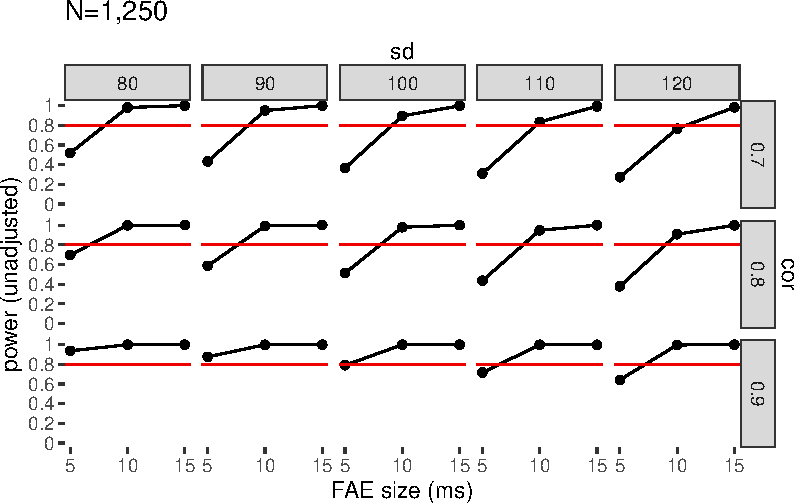
\includegraphics{index_files/figure-pdf/fig-power-1250-1.pdf}

}

\caption{\label{fig-power-1250}Power simulations with a sample size of
1,250, for all combinations of standard deviation (sd), pairwise
correlation (cor), and interaction effect size. The red line identifies
the threshold of 80\% power.}

\end{figure}%

\subsection{Methods}\label{sec-exp2-methods}

\subsubsection{Preregistration}\label{sec-exp2-prereg}

We preregistered the results of the power analysis, the goals, and the
design and analysis plan for experiment 2 prior to data collection. The
preregistration, containing the desired sample size, included variables,
hypotheses, and planned analyses is available on online
(\url{https://doi.org/10.17605/OSF.IO/3NFQP}).

\subsubsection{Materials}\label{sec-exp2-methods-materials}

One-hundred and four five-letter words, half of low frequency (between 7
and 24 in the SUBTLEX\(_{US}\) frequency per million) and half of high
frequency (between 57 and 2,961 in the SUBTLEX\(_{US}\) frequency per
million) were sampled from ELP (Balota et al. 2007), but this time based
on the SUBTLEX\(_{US}\) frequency counts rather than HAL as experiment
1. Table~\ref{tbl-words_exp2} shows that although the SUBTLEX\(_{US}\)
frequency ranges of the two conditions were very far from one another
(similarly to what was done in Experiment 1;
Section~\ref{sec-exp1-methods-materials}), they still show some overlap
in when HAL frequencies are used. As mentioned before, this seems to be
a general problem when considering different frequency databases at the
same time for a smaller set of stimuli that need to be manipulated and
controlled in different ways (see also fn. \ref{fn-databases}). From
each word set, fifty words were randomly chosen to be presented as
targets and related primes (the \emph{related} condition), and the
remaining fifty were presented as unrelated primes (the \emph{unrelated}
condition). All words used were monomorphemic nouns, adjectives, or
verbs, thus excluding particles, prepositions, and derived or inflected
forms.

\begin{longtable}{lrrrrrrrrr}

\caption{\label{tbl-words_exp2}Experiment 2. Descriptive statistics of
the word items used. For both frequency databases, the word frequencies
were converted to per-million count to ensure cross-comparison.}

\tabularnewline

\toprule
 &  & \multicolumn{4}{c}{\textbf{HAL}} & \multicolumn{4}{c}{\textbf{SUBTLEX\textsubscript{US}}} \\ 
\cmidrule(lr){3-6} \cmidrule(lr){7-10}
frequency & N & min & max & mean & SD & min & max & mean & SD \\ 
\midrule\addlinespace[2.5pt]
high & 52 & 45 & 4984 & 573 & 808 & 57 & 2691 & 210 & 388 \\ 
low & 52 & 6 & 570 & 64 & 93 & 7 & 24 & 13 & 5 \\ 
\bottomrule

\end{longtable}

One-hundred and four five-letter, phonotactically legal nonwords were
randomly selected from the ELP database as well. Half of them were
randomly selected to be presented as targets; the other half was instead
used as unrelated nonword primes. None of the nonwords contained any
existing English morpheme. Both the words and non-words used in the
experiments are reported in the appendix below.

\subsubsection{Participants}\label{sec-exp2-methods-participants}

Two thousand and six hundred participants (1445 females; age mean:
42.31; age sd: 14.12) were recruited on Prolific
(\url{https://www.prolific.com}) with the same criteria specified for
experiment 1 (Section~\ref{sec-exp1-methods-participants}).

\subsubsection{Procedure}\label{sec-exp2-methods-proc}

Experiment 2 was conducted in the same way as experiment 1 (see
Section~\ref{sec-exp1-methods-proc}). The median time to finish the
experiment was around 5 minutes.

\subsection{Data analysis}\label{sec-exp2-analysis}

Analysis scripts and an abridged version of the data collected can be
found online (\url{https://osf.io/vn3r2}), and consisted of 297,598
observations in total. We performed the same three steps of analysis
described for experiment 1 (Section~\ref{sec-exp1-analysis}).

\subsubsection{Step 1: subject and item
performance}\label{sec-exp2-analysis-performance}

Similarly to experiment 1, item and subject error rates were calculated.
The item error rate was never below above 14\%, so no item was excluded
from analysis. 19 subjects were removed because their error rate was
above 30\%. Thus, a total of 269,652 observations and 2,593 participants
were included in further analyses.

\subsubsection{Step 2: prime
durations}\label{sec-exp2-analysis-primeTime}

Prime fluctuations were dealt with in the same way as in experiment 1
(Section~\ref{sec-exp1-analysis-primeTime}). As compared to experiment
1, this time the mean (mean = 32.32 ms, sd = 15) and the median (median
= 33 ms) were closer to the intended prime duration (33 ms). The prime
duration cut-off set for experiment 1 (i.e., any trial whose prime
duration was out of the 25-60ms range) removed 13 \% of the trials. No
participant was excluded, for a total of 237,287 observations.

\subsubsection{Step 3: RT distribution}\label{sec-exp2-analysis-RT}

After removing the incorrect responses, similarly to what we did for
experiment 1 (Section~\ref{sec-exp1-analysis-RT}), 0.51\% of the trials
were excluded if the relative RT was below 200 ms and above 1800 ms,
Finally, 249 subjects were removed because the number of trials within
the same condition was less than 7 (i.e., about half of the total number
of trials being presented within the same condition, i.e.~13). A total
of 210,889 observations and 2,341 subjects were included in the
statistical analysis below.

\subsection{Results}\label{sec-exp2-results}

For each frequency condition, priming effects were calculated in the
same way as experiment 1. Table~\ref{tbl-exp2-statsResults} below report
the descriptive statistics of the experiment. All three conditions
showed statistically significant repetition priming effects
(\emph{MOP\_HF} = 18, CI\_95\% = {[}16 20{]}, t(2340) = 19.7,
\(p<.0001\); \emph{MOP\_LF} = 28, CI\_95\% = {[}26 30{]}, \emph{t}(2340)
= 27.8, \(p<.0001\); \emph{MOP\_NW} = -2, CI\_95\% = {[}-4 0{]}, t(2340)
= -2.33, \(p<.0001\)). The low-frequency word repetition priming effect
was 10 ms larger than the high-frequency word repetition priming effect,
and this FAE effect was statistically significant (\emph{M\_FAE} = 10,
CI\_95\% = {[}7 13{]}), \emph{t}(2340) = 7.24, \(p<.0001\)). As for the
word error analysis, we found significant priming effects in the word
conditions (high: \emph{t}(2340)=9.95, \emph{p}\textless.0001; low:
\emph{t}(2340)=16.9, \emph{p}\textless.0001), as well as in the non-word
condition (non-word: \emph{t}(2340)=-3.27, \emph{p}=.001).

\blandscape

\begin{longtable}{lrrrrrrrrlrrrrl}

\caption{\label{tbl-exp2-statsResults}Experiment 2. Summary of the word
priming results. \emph{Legend.} MOP: magnitude of priming.}

\tabularnewline

\toprule
 & \multicolumn{3}{c}{unrelated RT} & \multicolumn{3}{c}{repetition RT} &  & \multicolumn{4}{c}{priming effects} & \multicolumn{3}{c}{\emph{t}-test} \\ 
\cmidrule(lr){2-4} \cmidrule(lr){5-7} \cmidrule(lr){9-12} \cmidrule(lr){13-15}
factor & mean & SD & Error (\%) & mean & SD & Error (\%) & cor & MOP & 95\% CI & SD\textsubscript{p} & ES & \emph{t} & df & \emph{p} \\ 
\midrule\addlinespace[2.5pt]
high & 573 & 83 & 3 & 555 & 85 & 2 & 0.860 & 18 & [16 20] & 45 & 0.41 & 19.7 & 2340 & 2.88e-80 \\ 
low & 605 & 88 & 6 & 577 & 88 & 3 & 0.850 & 28 & [26 30] & 49 & 0.58 & 27.8 & 2340 & 1.52e-147 \\ 
non-word & 623 & 103 & 4 & 625 & 103 & 4 & 0.910 & -2 & [-4 0] & 43 & -0.05 & -2.33 & 2340 & 0.0197 \\ 
frequency:primetype &   &   &   &   &   &   & 0.029 & 10 & [7 13] & 66 & 0.15 & 7.24 & 2340 & 5.86e-13 \\ 
\bottomrule

\end{longtable}

\elandscape

\subsection{Discussion}\label{sec-exp2-discussion}

Experiment 2 was specifically designed to investigate the replicability
of the Frequency Attenuation Effect (FAE) observed in an unmasked
environment (i.e., with a SOA \textgreater{} 60 ms) within the confines
of a masked environment (with SOA \textless{} 60 ms). We employed a
robust sample size to ensure adequate statistical power for detecting
small to medium effect sizes. Our results not only replicated Experiment
1 in revealing significant main effects of repetition for high and low
frequency words alike, but also detected a statistically significant
interaction: the low-frequency condition manifested priming effects that
were found approximately 9 ms bigger than the high-frequency condition.

The non-word masked priming response (or lack thereof) has been used as
an additional piece of evidence in favor of the vision of the masked
priming response as devoid of episodic influences (e.g., Forster 1999).
The results of experiment 2 align with the past evidence in showing no
significant (inhibitory) masked repetition priming for non-words.
However, we will not further delve into this topic here, as it does not
strictly impinge on the question being asked here (i.e., word frequency
effects in masked priming), and would deserve a full-fledged
investigation on its own right.

\section{General discussion}\label{sec-discussion}

The repetition priming response stands as a cornerstone in
psycholinguistic investigations, offering insights into the mechanisms
governing word recognition. An ongoing debate surrounds the
interpretation of these effects, particularly concerning their source in
the memory system. On the one hand, \emph{interactive activation models}
(McClelland and Rumelhart 1981; Grainger and Jacobs 1996; Coltheart et
al. 2001) posit a lexical source for repetition priming effects, either
in terms of temporarily raised resting activation levels for lexical
nodes in unmasked priming, or as a head start in the retrieval process
in masked priming. \emph{Episodic} and \emph{memory recruitment models}
(Jacoby and Dallas 1981; Jacoby 1983; Bodner and Masson 1997; Masson and
Bodner 2003; Bodner and Masson 2014) on the other hand, invoke a
non-lexical source for the repetition effect, namely an episodic or
episodic-like memory resource formed upon brief exposure to the prime
word that can be recruited during the processing of the target item.
Crucially, both models predict a single mechanism underlying masked and
unmasked priming. Differential mechanisms between unmasked and masked
repetition priming, however, are predicted by the \emph{entry-opening
model} (Forster and Davis 1984), which propose both lexical and episodic
sources of priming effects.

Thus, the existence of qualitatively distinct outcomes in masked and
unmasked priming presented a direct challenge to some, but not all of
these models. One such finding is the \emph{Frequency Attenuation
Effect} (FAE), in which higher frequency words exhibit smaller
repetition effects compared to lower frequency words. The FAE has been
described as observable only in unmasked priming since the work of
Forster and Davis (1984), who demonstrated that when the prime word is
presented very briefly (SOA \(<\) 60 ms), it becomes masked by the
target word, and this prevents the conscious encoding of the prime.
Under such conditions, the FAE purportedly disappears. Forster and Davis
(1984) argued that this potentially shows that the FAE is subserved by a
different type of memory source (perhaps episodic) than the masked
repetition priming response. This conclusion, however, is the source of
ongoing debates (see Table~\ref{tbl-litReview} for review of past
findings), which the two experiments reported here were meant to
address.

Within this research landscape, our experiments targeting the frequency
sensitivity of the repetition effect under masked conditions contribute
methodological and theoretical insights. Methodologically, our results
help establish the viability and reliability of online data collection
for the masked priming paradigm. Building on the pioneering work of
Angele et al. (2023) and Cayado, Wray, and Stockall (2023), we addressed
pitfalls in implementing and analyzing masked priming data collected
online, and by doing so offered a solution to the longstanding problem
of low statistical power involving investigating phenomena with effect
sizes that are harder to detect statistically, like interactions in
factorial designs. However, this newfound opportunity necessitates
careful data scrutiny, as demonstrated by significant data loss due to
stringent exclusion criteria in experiments 1 and 2 (30\% to 60\% of the
total data), highlighting the need for further exploration of less
restrictive criteria and their impact on data quality.

In the same vein, the significant FAE observed in Experiment 2 has
important theoretical ramifications. The historical belief in the
non-observability of FAE in masked priming primarily arose from a lack
of statistically significant results, possibly rooted in outdated
frequency corpora or inadequate statistical power. Our design addressed
these concerns, yielding statistically significant FAE results aligning
with the literature's average effect (see Table~\ref{tbl-litReview}; the
95\% CI implies that the FAE is unlikely to be larger than 17 ms with a
33 ms prime duration). These results challenge the supposed qualitative
distinction between masked and unmasked repetition priming cleaved by
the FAE, complicating the rejection of single-mechanism theories, and
suggesting that \emph{interactive-activation models} and \emph{memory
recruitment models} may yet offer unifying explanations for masked and
unmasked priming.

Similarly, our results also challenge the entry-opening model's
prediction of the absence of FAE in masked priming. One potential way of
dealing with this in the \emph{entry opening model} is to claim that
masked priming severely reduces, but does not entirely eliminate, the
use of sources other than lexical memory (see Forster 1998; Forster,
Mohan, and Hector 2003, for proposals along this line). Alternatively,
within the entry-opening model, the results of experiment 2 may be
explained by the frequency-based mechanism occurring in the fast search
stage. A potential mechanism in this direction was already hinted at by
Forster and Davis (1984) themselves, and consists of a procedure,
whereby during the fast search stage, the entry of a prime word is
promoted to the top position of the search list. As a consequence,
low-frequency words (which are fairly low in the search list) will
benefit from such promotion procedure more than high-frequency words
(which are instead already in higher positions), thus ultimately giving
rise to the FAE.

While our findings present a compelling case for the presence of FAE in
masked priming that is seemingly parallel to the unmasked case,
questions about potential mechanistic differences persist. The larger
sample size needed for masked FAEs raises intriguing considerations
about the influence of memory sources and warrants further
investigation. Additionally, the absence of significant non-word priming
in experiment 2 aligns with the trend (overwhelmingly shown in the
literature) that it may be exclusive to unmasked designs (Forster 1998;
Forster, Mohan, and Hector 2003; but see Masson and Bodner 2003), and
suggests avenues for future exploration on large-scale.

Finally, the finding that the FAE occurs under masked priming conditions
may impact our understanding of masked morphological priming. In this
literature, there is a unresolved question about the ability of affixes
to elicit masked morphological priming results (for a review, Amenta and
Crepaldi 2012). In English, the evidence seems to indicate that only
stems, but not affixes, have the ability to prime entries across the
lexicon. This finding can and has been used to support models in which
affixes are initially stripped before stems are accessed in the lexicon
(Taft and Forster 1975; Forster and Azuma 2000; Stockall and Marantz
2006). However, stems and affixes do also have a large frequency
imbalance, with most affixes being substantially more frequent that most
stems. The observation of FAE under masked priming can provide an
alternative reason for why masked stem morphological priming is well
attested but masked affix morphological priming is not: the latter could
be due to a ceiling frequency attenuation effect. This is an intriguing
possibility that must be left for future work to explore.

In summary, our study successfully replicated and expanded upon the work
of Angele et al. (2023) and Cayado, Wray, and Stockall (2023),
confirming the viability of observing repetition priming effects in
masked priming experiments conducted online with a brief Stimulus Onset
Asynchrony (SOA) of 33 ms. Notably, we addressed a lingering question in
the literature by establishing the presence of the Frequency Attenuation
Effect (FAE) under masked conditions. The use of large online samples
proved instrumental in overcoming the longstanding challenge of
insufficient statistical power to detect interactions in factorial
designs, which we believe had impeded previous investigations into
detecting the FAE in masked priming.

These results not only contribute to our understanding of masked priming
but also open up intriguing avenues for further research. The ability to
harness extensive online samples provides a valuable opportunity to
explore and illuminate unresolved issues across various domains where
masked priming is a crucial research tool, underscoring the potential
for online experimentation to advance our knowledge and resolve
long-standing questions in the field.

\section*{References}\label{references}
\addcontentsline{toc}{section}{References}

\phantomsection\label{refs}
\begin{CSLReferences}{1}{0}
\bibitem[\citeproctext]{ref-AmentaCrepaldi2012}
Amenta, Simona, and Davide Crepaldi. 2012. {``Morphological Processing
as We Know It: An Analytical Review of Morphological Effects in Visual
Word Identification.''} \emph{Frontiers in Psychology} 3: 232.

\bibitem[\citeproctext]{ref-Angele2023}
Angele, Bernhard, Ana Baciero, Pablo Gómez, and Manuel Perea. 2023.
{``Does Online Masked Priming Pass the Test? The Effects of Prime
Exposure Duration on Masked Identity Priming.''} \emph{Behavior Research
Methods} 55 (1): 151--67.
\url{https://doi.org/10.3758/s13428-021-01742-y}.

\bibitem[\citeproctext]{ref-Anwyl2020}
Anwyl-Irvine, Alexander L, Jessica Massonnié, Adam Flitton, Natasha
Kirkham, and Jo K Evershed. 2020. {``Gorilla in Our Midst: An Online
Behavioral Experiment Builder.''} \emph{Behavior Research Methods} 52:
388--407.

\bibitem[\citeproctext]{ref-Balota2004}
Balota, David A., Michael J. Cortese, Susan D. Sergent-Marshall, Daniel
H. Spieler, and Melvin J. Yap. 2004. {``Visual Word Recognition of
Single-Syllable Words.''} \emph{Journal of Experimental Psychology:
General} 133 (2): 283.

\bibitem[\citeproctext]{ref-balota2007}
Balota, David A., Melvin J. Yap, Keith A. Hutchison, Michael J. Cortese,
Brett Kessler, Bjorn Loftis, James H. Neely, Douglas L. Nelson, Greg B.
Simpson, and Rebecca Treiman. 2007. {``The English Lexicon Project.''}
\emph{Behavior Research Methods} 39 (3): 445--59.
\url{https://doi.org/10.3758/bf03193014}.

\bibitem[\citeproctext]{ref-Bodner2014}
Bodner, Glen E., and Michael E. J Masson. 2014. {``Memory Recruitment: A
Backward Idea about Masked Priming.''} In \emph{Psychology of Learning
and Motivation}, 61:179--213. Elsevier.

\bibitem[\citeproctext]{ref-BodnerMasson1997}
Bodner, Glen E., and Michael E. J. Masson. 1997. {``Masked Repetition
Priming of Words and Nonwords: Evidence for a Nonlexical Basis for
Priming.''} \emph{Journal of Memory and Language} 37 (2): 268--93.
\url{https://doi.org/10.1006/jmla.1996.2507}.

\bibitem[\citeproctext]{ref-BodnerMasson2001}
---------. 2001. {``Prime Validity Affects Masked Repetition Priming:
Evidence for an Episodic Resource Account of Priming.''} \emph{Journal
of Memory and Language} 45 (4): 616--47.
\url{https://doi.org/10.1006/jmla.2001.2791}.

\bibitem[\citeproctext]{ref-Brysbaert2011}
Brysbaert, Marc, and Michael J Cortese. 2011. {``Do the Effects of
Subjective Frequency and Age of Acquisition Survive Better Word
Frequency Norms?''} \emph{Quarterly Journal of Experimental Psychology}
64 (3): 545--59.

\bibitem[\citeproctext]{ref-Brysbaert2018}
Brysbaert, Marc, Paweł Mandera, and Emmanuel Keuleers. 2018. {``The Word
Frequency Effect in Word Processing: An Updated Review.''} \emph{Current
Directions in Psychological Science} 27 (1): 45--50.

\bibitem[\citeproctext]{ref-BrysbaertNew2009}
Brysbaert, Marc, and Boris New. 2009. {``Moving Beyond Ku{č}era and
Francis: A Critical Evaluation of Current Word Frequency Norms and the
Introduction of a New and Improved Word Frequency Measure for American
English.''} \emph{Behavior Research Methods} 41 (4): 977--90.
\url{https://doi.org/10.3758/brm.41.4.977}.

\bibitem[\citeproctext]{ref-BrysbaertStevens2018}
Brysbaert, Marc, and Michaël Stevens. 2018. {``Power Analysis and Effect
Size in Mixed Effects Models: A Tutorial.''} \emph{Journal of Cognition}
1 (1). \url{https://doi.org/10.5334/joc.10}.

\bibitem[\citeproctext]{ref-Burgess1998}
Burgess, Curt, and Kay Livesay. 1998. {``The Effect of Corpus Size in
Predicting Reaction Time in a Basic Word Recognition Task: Moving on
from Ku{č}era and Francis.''} \emph{Behavior Research Methods,
Instruments, \& Computers} 30 (2): 272--77.

\bibitem[\citeproctext]{ref-Button2013}
Button, Katherine S, John PA Ioannidis, Claire Mokrysz, Brian A Nosek,
Jonathan Flint, Emma SJ Robinson, and Marcus R Munafò. 2013. {``Power
Failure: Why Small Sample Size Undermines the Reliability of
Neuroscience.''} \emph{Nature Reviews Neuroscience} 14 (5): 365--76.

\bibitem[\citeproctext]{ref-Cayado2023}
Cayado, Dave Kenneth Tayao, Samantha Wray, and Linnaea Stockall. 2023.
{``Does Linear Position Matter for Morphological Processing? Evidence
from a Tagalog Masked Priming Experiment.''} \emph{Language, Cognition
and Neuroscience}, 1--16.

\bibitem[\citeproctext]{ref-Cohen1992}
Cohen, Jacob. 1992. {``A Power Primer.''} \emph{Psychological Bulletin}
112 (1): 155--59. \url{https://doi.org/10.1037/0033-2909.112.1.155}.

\bibitem[\citeproctext]{ref-ColtheartEtal2001}
Coltheart, Max, Kathleen Rastle, Conrad Perry, Robyn Langdon, and
Johannes Ziegler. 2001. {``DRC: A Dual Route Cascaded Model of Visual
Word Recognition and Reading Aloud.''} \emph{Psychological Review} 108
(1): 204--56.

\bibitem[\citeproctext]{ref-EvettHumphreys1981}
Evett, Lindsay J., and Glyn W. Humphreys. 1981. {``The Use of Abstract
Graphemic Information in Lexical Access.''} \emph{The Quarterly Journal
of Experimental Psychology} 33 (4): 325--50.

\bibitem[\citeproctext]{ref-Labvanced2017}
Finger, Holger, Caspar Goeke, Dorena Diekamp, Kai Standvoß, and Peter
König. 2017. {``LabVanced: A Unified JavaScript Framework for Online
Studies.''} In \emph{2017 International Conference on Computational
Social Science}. Cologne, Germany.

\bibitem[\citeproctext]{ref-Forster1998}
Forster, Kenneth I. 1998. {``The Pros and Cons of Masked Priming.''}
\emph{Journal of Psycholinguistic Research} 27 (2): 203--33.

\bibitem[\citeproctext]{ref-Forster1999}
---------. 1999. {``Microgenesis of Priming Effects in Lexical
Access.''} \emph{Brain and Language} 68: 5--15.

\bibitem[\citeproctext]{ref-ForsterAzuma2000}
Forster, Kenneth I., and Tamiko Azuma. 2000. {``Masked Priming for
Prefixed Words with Bound Stems: Does Submit Prime Permit?''}
\emph{Language and Cognitive Processes} 15 (4-5): 539--61.

\bibitem[\citeproctext]{ref-ForsterDavis1984}
Forster, Kenneth I., and Chris Davis. 1984. {``Repetition Priming and
Frequency Attenuation in Lexical Access.''} \emph{Journal of
Experimental Psychology: Learning, Memory, and Cognition} 10 (4): 680.

\bibitem[\citeproctext]{ref-ForsterDavis1991}
Forster, Kenneth I., and Christopher Davis. 1991. {``The Density
Constraint on Form-Priming in the Naming Task: Interference Effects from
a Masked Prime.''} \emph{Journal of Memory and Language} 30 (1): 1--25.
\url{https://doi.org/10.1016/0749-596x(91)90008-8}.

\bibitem[\citeproctext]{ref-ForsterEtal1987}
Forster, Kenneth I., C. Davis, C. Schoknecht, and R. Carter. 1987.
{``Masked Priming with Graphemically Related Forms: Repetition or
Partial Activation?''} \emph{The Quarterly Journal of Experimental
Psychology Section A} 39 (2): 211--51.
\url{https://doi.org/10.1080/14640748708401785}.

\bibitem[\citeproctext]{ref-ForsterEtal2003}
Forster, Kenneth I., Kathleen Mohan, and Jo Hector. 2003. {``The
Mechanics of Masked Priming.''} In \emph{Masked Priming: The State of
the Art}, edited by Sachiko Kinoshita and Stephen J. Lupker, 3--37. New
York, NY/Hove, UK: Psychology Press.

\bibitem[\citeproctext]{ref-GelmanCarlin2014}
Gelman, Andrew, and John Carlin. 2014. {``Beyond Power Calculations.''}
\emph{Perspectives on Psychological Science} 9 (6): 641--51.
\url{https://doi.org/10.1177/1745691614551642}.

\bibitem[\citeproctext]{ref-Gimenes2016}
Gimenes, Manuel, and Boris New. 2016. {``Worldlex: Twitter and Blog Word
Frequencies for 66 Languages.''} \emph{Behavior Research Methods} 48:
963--72.

\bibitem[\citeproctext]{ref-GraingerJacobs1996}
Grainger, Jonathan, and Arthur M. Jacobs. 1996. {``Orthographic
Processing in Visual Word Recognition: A Multiple Read-Out Model.''}
\emph{Psychological Review} 103 (3): 518.

\bibitem[\citeproctext]{ref-Herdaugdelen2017}
Herdağdelen, Amaç, and Marco Marelli. 2017. {``Social Media and Language
Processing: How Facebook and Twitter Provide the Best Frequency
Estimates for Studying Word Recognition.''} \emph{Cognitive Science} 41
(4): 976--95.

\bibitem[\citeproctext]{ref-Jacoby1983}
Jacoby, Larry L. 1983. {``Remembering the Data: Analyzing Interactive
Processes in Reading.''} \emph{Journal of Verbal Learning and Verbal
Behavior} 22 (5): 485--508.

\bibitem[\citeproctext]{ref-Jacoby1981}
Jacoby, Larry L, and Mark Dallas. 1981. {``On the Relationship Between
Autobiographical Memory and Perceptual Learning.''} \emph{Journal of
Experimental Psychology: General} 110 (3): 306.

\bibitem[\citeproctext]{ref-Kinoshita2006}
Kinoshita, Sachiko. 2006. {``Additive and Interactive Effects of Word
Frequency and Masked Repetition in the Lexical Decision Task.''}
\emph{Psychonomic Bulletin \& Review} 13 (4): 668--73.
\url{https://doi.org/10.3758/bf03193979}.

\bibitem[\citeproctext]{ref-KuceraFrancis1967}
Kučera, J., and W. N. Francis. 1967. \emph{Computational Analysis of
Present Day American English}. Providence, RI: Brown University Press.

\bibitem[\citeproctext]{ref-deLeeuw2014}
Leeuw, Joshua R. de. 2014. {``jsPsych: A JavaScript Library for Creating
Behavioral Experiments in a Web Browser.''} \emph{Behavior Research
Methods} 47 (1): 1--12. \url{https://doi.org/10.3758/s13428-014-0458-y}.

\bibitem[\citeproctext]{ref-LukacsGaspar2023}
Lukács, Gáspár, and Andreas Gartus. 2023. {``Precise Display Time
Measurement in JavaScript for Web-Based Experiments.''} \emph{Behavior
Research Methods} 55 (3): 1079--93.
\url{https://doi.org/10.3758/s13428-022-01835-2}.

\bibitem[\citeproctext]{ref-LundBurgess1996}
Lund, Kevin, and Curt Burgess. 1996. {``Producing High-Dimensional
Semantic Spaces from Lexical Co-Occurrence.''} \emph{Behavior Research
Methods, Instruments, {\&} Computers} 28 (2): 203--8.

\bibitem[\citeproctext]{ref-MassonBodner2003}
Masson, Michael E. J., and Glen E. Bodner. 2003. {``A Retrospective View
of Masked Priming: Toward a Unified Account of Masked and Long-Term
Repetition Priming.''} \emph{Masked Priming: The State of the Art},
57--94.

\bibitem[\citeproctext]{ref-McClellandRumelhart1981}
McClelland, James L., and David E. Rumelhart. 1981. {``An Interactive
Activation Model of Context Effects in Letter Perception: Part i. An
Account of Basic Findings.''} \emph{Psychological Review} 88 (5):
375--407.

\bibitem[\citeproctext]{ref-Nievas2010}
Nievas, Francisco. 2010. {``The Frequency Attenuation Effect in Identity
and Associative Priming.''} \emph{The Spanish Journal of Psychology} 13
(1): 30--62. \url{https://doi.org/10.1017/s1138741600003668}.

\bibitem[\citeproctext]{ref-NorrisKinoshita2008}
Norris, Dennis, and Sachiko Kinoshita. 2008. {``Perception as Evidence
Accumulation and Bayesian Inference: Insights from Masked Priming.''}
\emph{Journal of Experimental Psychology: General} 137 (3): 434--55.
\url{https://doi.org/10.1037/a0012799}.

\bibitem[\citeproctext]{ref-PeirceEtal2019}
Peirce, Jonathan, Jeremy R. Gray, Sol Simpson, Michael MacAskill,
Richard Höchenberger, Hiroyuki Sogo, Erik Kastman, and Jonas Kristoffer
Lindeløv. 2019. {``PsychoPy2: Experiments in Behavior Made Easy.''}
\emph{Behavior Research Methods} 51 (1): 195--203.

\bibitem[\citeproctext]{ref-Petrosino2020}
Petrosino, Roberto. 2020. {``More Than Islands of Regularity: An
Investigation of the Sensitivity of Morphological Decomposition to
Higher-Level Linguistic Properties.''} PhD thesis, University of
Connecticut.

\bibitem[\citeproctext]{ref-PetrosinoEtal2023}
Petrosino, Roberto, Jon Sprouse, and Diogo Almeida. 2023. {``Asymmetries
in the Stem and Suffix Masked Priming Response in a Large-Scale Online
Study.''} \emph{Quaderni Di Linguistica e Studi Orientali}, no. 49:
177--94. \url{https://doi.org/10.13128/QUL-SO-2421-7220-15154}.

\bibitem[\citeproctext]{ref-PotvinSchtuz2000}
Potvin, Patrick J., and Robert W. Schutz. 2000. {``Statistical Power for
the Two-Factor Repeated Measures ANOVA.''} \emph{Behavior Research
Methods, Instruments, \& Computers} 32 (2): 347--56.
\url{https://doi.org/10.3758/bf03207805}.

\bibitem[\citeproctext]{ref-RajaramNeely1992}
Rajaram, Suparna, and James H Neely. 1992. {``Dissociative Masked
Repetition Priming and Word Frequency Effects in Lexical Decision and
Episodic Recognition Tasks.''} \emph{Journal of Memory and Language} 31
(2): 152--82. \url{https://doi.org/10.1016/0749-596x(92)90009-m}.

\bibitem[\citeproctext]{ref-ScarboroughEtal1977}
Scarborough, Don L., Charles Cortese, and Hollis S. Scarborough. 1977.
{``Frequency and Repetition Effects in Lexical Memory.''} \emph{Journal
of Experimental Psychology: Human Perception and Performance} 3 (1):
1--17. \url{https://doi.org/10.1037/0096-1523.3.1.1}.

\bibitem[\citeproctext]{ref-SeguiGrainger1990}
Segui, Juan, and Jonathan Grainger. 1990. {``Priming Word Recognition
with Orthographic Neighbors: Effects of Relative Prime-Target
Frequency.''} \emph{Journal of Experimental Psychology: Human Perception
and Performance} 16 (1): 65--76.
\url{https://doi.org/10.1037/0096-1523.16.1.65}.

\bibitem[\citeproctext]{ref-Sereno1991}
Sereno, Joan A. 1991. {``Graphemic, Associative, and Syntactic Priming
Effects at a Brief Stimulus Onset Asynchrony in Lexical Decision and
Naming.''} \emph{Journal of Experimental Psychology: Learning, Memory,
and Cognition} 17 (3): 459--77.
\url{https://doi.org/10.1037/0278-7393.17.3.459}.

\bibitem[\citeproctext]{ref-StockallMarantz2006}
Stockall, Linnaea, and Alec Marantz. 2006. {``A Single Route, Full
Decomposition Model of Morphological Complexity: MEG Evidence.''}
\emph{The Mental Lexicon} 1 (1): 85--123.
https://doi.org/\url{https://doi.org/10.1075/ml.1.1.07sto}.

\bibitem[\citeproctext]{ref-TaftForster1975}
Taft, Marcus, and Kenneth I. Forster. 1975. {``Lexical Storage and
Retrieval of Prefixed Words.''} \emph{Journal of Verbal Learning and
Verbal Behavior} 14 (6): 638--47.

\bibitem[\citeproctext]{ref-Yap2009}
Yap, Melvin J., and David A. Balota. 2009. {``Visual Word Recognition of
Multisyllabic Words.''} \emph{Journal of Memory and Language} 60 (4):
502--29.

\bibitem[\citeproctext]{ref-Zevin2002}
Zevin, Jason D, and Mark S Seidenberg. 2002. {``Age of Acquisition
Effects in Word Reading and Other Tasks.''} \emph{Journal of Memory and
Language} 47 (1): 1--29.

\end{CSLReferences}

\newpage

\section*{Wordlists}\label{wordlists}
\addcontentsline{toc}{section}{Wordlists}

\subsubsection*{Experiment 1}\label{experiment-1}
\addcontentsline{toc}{subsubsection}{Experiment 1}

\begin{longtable*}{llrrrr}
\toprule
 &  & \multicolumn{2}{c}{RT (to repetition)} & \multicolumn{2}{c}{RT (to unrelated)} \\ 
\cmidrule(lr){3-4} \cmidrule(lr){5-6}
unrelated prime & word & mean & SD & mean & SD \\ 
\midrule\addlinespace[2.5pt]
\multicolumn{6}{l}{\emph{low frequency condition}} \\ 
\midrule\addlinespace[2.5pt]
smash & chasm & 714 & 216 & 831 & 250 \\ 
manna & oxide & 719 & 198 & 715 & 156 \\ 
legit & vowel & 655 & 139 & 694 & 152 \\ 
blunt & clerk & 617 & 157 & 635 & 133 \\ 
slope & bleed & 609 & 171 & 621 & 176 \\ 
nasal & decor & 654 & 140 & 694 & 204 \\ 
forte & quirk & 689 & 204 & 688 & 155 \\ 
aloud & speck & 732 & 208 & 739 & 187 \\ 
nymph & stash & 638 & 175 & 657 & 142 \\ 
crass & ditch & 671 & 173 & 678 & 157 \\ 
squid & snare & 684 & 168 & 722 & 164 \\ 
swirl & budge & 672 & 200 & 732 & 207 \\ 
grunt & slack & 608 & 129 & 664 & 157 \\ 
taunt & sedan & 711 & 197 & 705 & 122 \\ 
cigar & tally & 667 & 131 & 720 & 176 \\ 
lunge & posit & – & – & – & – \\ 
negro & flock & 654 & 141 & 716 & 166 \\ 
exert & scorn & 670 & 159 & 651 & 146 \\ 
lathe & grail & 697 & 206 & 718 & 171 \\ 
viola & bloat & 663 & 185 & 698 & 181 \\ 
rival & tumor & 627 & 159 & 651 & 152 \\ 
dizzy & acute & 662 & 174 & 660 & 142 \\ 
hertz & sauna & 652 & 132 & 706 & 154 \\ 
haste & elect & 640 & 162 & 650 & 144 \\ 
poppy & spoof & 706 & 185 & 759 & 201 \\ 
clove & plush & 615 & 138 & 669 & 175 \\ 
guise & fiend & 785 & 209 & 846 & 185 \\ 
magma & knelt & 744 & 213 & 814 & 225 \\ 
lotto & privy & 733 & 182 & 777 & 219 \\ 
kayak & sigma & 798 & 258 & 796 & 205 \\ 
taint & parse & – & – & – & – \\ 
fanny & carte & – & – & – & – \\ 
rouge & verge & 664 & 168 & 672 & 171 \\ 
vitro & mourn & 665 & 171 & 682 & 186 \\ 
floss & shrug & 687 & 175 & 682 & 132 \\ 
tempt & clasp & 658 & 128 & 701 & 178 \\ 
flirt & bathe & 659 & 159 & 701 & 197 \\ 
fluff & linen & 620 & 91 & 650 & 133 \\ 
butch & stare & 617 & 126 & 632 & 144 \\ 
bowel & medic & 637 & 166 & 663 & 218 \\ 
aspen & weave & 614 & 128 & 649 & 128 \\ 
chime & flint & 681 & 140 & 718 & 191 \\ 
crust & flank & 689 & 176 & 740 & 177 \\ 
spunk & scrub & 645 & 172 & 670 & 167 \\ 
stoke & hoist & 686 & 168 & 724 & 190 \\ 
dairy & stout & 667 & 148 & 707 & 166 \\ 
stale & cough & 588 & 147 & 629 & 157 \\ 
gypsy & annex & 744 & 197 & 798 & 169 \\ 
gloss & plume & 730 & 195 & 775 & 194 \\ 
topaz & quart & 662 & 159 & 715 & 205 \\ 
\midrule\addlinespace[2.5pt]
\multicolumn{6}{l}{\emph{high frequency condition}} \\ 
\midrule\addlinespace[2.5pt]
shoot & proof & 576 & 119 & 617 & 129 \\ 
usual & clear & 598 & 169 & 588 & 120 \\ 
teach & audio & 589 & 141 & 632 & 112 \\ 
adult & apply & 592 & 154 & 632 & 130 \\ 
allow & phone & 573 & 143 & 588 & 89 \\ 
forum & class & 656 & 162 & 682 & 197 \\ 
whole & raise & 611 & 154 & 598 & 116 \\ 
often & civil & 580 & 107 & 623 & 120 \\ 
issue & match & 590 & 119 & 619 & 169 \\ 
style & local & 589 & 141 & 580 & 113 \\ 
coast & minor & 600 & 137 & 632 & 157 \\ 
reach & below & 611 & 143 & 618 & 90 \\ 
smith & extra & 599 & 146 & 609 & 141 \\ 
speed & court & 585 & 115 & 638 & 141 \\ 
sense & exact & 592 & 127 & 590 & 113 \\ 
write & bunch & 647 & 140 & 646 & 130 \\ 
trust & quick & 554 & 104 & 616 & 134 \\ 
sleep & birth & 619 & 165 & 609 & 156 \\ 
reply & truth & 579 & 140 & 611 & 150 \\ 
track & serve & 611 & 136 & 649 & 168 \\ 
dream & trade & 606 & 185 & 602 & 106 \\ 
image & heart & 592 & 159 & 602 & 113 \\ 
white & index & 606 & 111 & 625 & 146 \\ 
flame & cable & 583 & 119 & 626 & 130 \\ 
value & break & 605 & 163 & 601 & 133 \\ 
avoid & woman & 576 & 119 & 609 & 153 \\ 
short & front & 587 & 138 & 619 & 140 \\ 
aware & voice & 562 & 127 & 585 & 116 \\ 
large & stock & 596 & 148 & 661 & 216 \\ 
prove & seven & 583 & 130 & 653 & 193 \\ 
brand & blood & 568 & 109 & 598 & 109 \\ 
river & plain & 596 & 115 & 617 & 123 \\ 
guess & solid & 643 & 158 & 612 & 140 \\ 
month & limit & 603 & 122 & 658 & 136 \\ 
heard & scale & 632 & 144 & 639 & 176 \\ 
space & stuff & 623 & 133 & 642 & 154 \\ 
leave & major & 599 & 139 & 585 & 123 \\ 
agree & brown & 591 & 120 & 632 & 167 \\ 
metal & house & 552 & 121 & 603 & 137 \\ 
along & stage & 590 & 138 & 619 & 160 \\ 
print & built & 628 & 155 & 664 & 166 \\ 
worst & video & 570 & 113 & 650 & 157 \\ 
sound & story & 594 & 129 & 614 & 176 \\ 
faith & march & 607 & 134 & 630 & 191 \\ 
quote & clean & 553 & 93 & 585 & 135 \\ 
train & price & 599 & 141 & 624 & 189 \\ 
small & event & 583 & 127 & 623 & 166 \\ 
night & thank & 656 & 190 & 607 & 128 \\ 
shell & radio & 577 & 131 & 604 & 162 \\ 
alone & sorry & 592 & 155 & 609 & 140 \\ 
\midrule\addlinespace[2.5pt]
\multicolumn{6}{l}{non-word} \\ 
\midrule\addlinespace[2.5pt]
strat & inurt & 726 & 259 & 712 & 215 \\ 
gleat & shawt & 760 & 270 & 672 & 154 \\ 
dolio & delax & 758 & 182 & 767 & 195 \\ 
cutch & thelp & 745 & 242 & 687 & 199 \\ 
greaf & isapt & 645 & 181 & 628 & 160 \\ 
broot & fopaz & 660 & 196 & 628 & 125 \\ 
lubic & fuxom & 676 & 234 & 601 & 126 \\ 
drirk & bloot & 761 & 190 & 744 & 172 \\ 
cooch & scart & 768 & 220 & 726 & 162 \\ 
motem & frint & 720 & 203 & 685 & 148 \\ 
abapt & ahuck & 673 & 207 & 633 & 153 \\ 
nigit & netro & 734 & 217 & 721 & 169 \\ 
hilac & moust & 744 & 186 & 798 & 174 \\ 
cojex & barsh & 731 & 216 & 706 & 183 \\ 
prilt & avort & 710 & 196 & 725 & 199 \\ 
whirp & venem & – & – & – & – \\ 
shino & grack & 743 & 209 & 728 & 182 \\ 
nelch & ranth & 681 & 174 & 654 & 135 \\ 
exulk & frick & – & – & – & – \\ 
morex & nohew & 683 & 197 & 656 & 165 \\ 
tamek & pramp & 745 & 239 & 696 & 200 \\ 
miant & altep & 664 & 179 & 654 & 159 \\ 
bloth & scrib & 788 & 243 & 749 & 230 \\ 
bumbo & tumph & 785 & 204 & 768 & 210 \\ 
occut & dorst & 686 & 168 & 674 & 184 \\ 
topec & thint & 754 & 205 & 748 & 153 \\ 
shoof & rourt & 691 & 192 & 688 & 194 \\ 
spack & smout & 759 & 195 & 736 & 184 \\ 
blenk & kayuk & 823 & 289 & 772 & 237 \\ 
silaf & drick & 727 & 189 & 678 & 131 \\ 
crunk & smoop & 710 & 185 & 684 & 154 \\ 
fluck & deirm & 649 & 161 & 657 & 178 \\ 
ghisk & ephic & 787 & 223 & 751 & 212 \\ 
chrik & glurp & 731 & 209 & 727 & 236 \\ 
cetup & blumb & 746 & 183 & 733 & 220 \\ 
firch & eicht & 725 & 226 & 718 & 205 \\ 
vasem & forim & 736 & 214 & 690 & 185 \\ 
earch & slent & 840 & 207 & 773 & 178 \\ 
blont & lepot & 693 & 203 & 659 & 162 \\ 
ecret & plock & 763 & 222 & 734 & 195 \\ 
wateb & ocheb & 643 & 168 & 620 & 130 \\ 
trook & febut & 659 & 166 & 632 & 156 \\ 
ruzak & coreb & 656 & 169 & 643 & 133 \\ 
theet & frath & 738 & 193 & 699 & 148 \\ 
blamp & eggem & 705 & 190 & 681 & 160 \\ 
lambo & gredo & 700 & 217 & 689 & 182 \\ 
aliom & brost & 728 & 204 & 690 & 170 \\ 
brust & ganic & 712 & 178 & 660 & 117 \\ 
cleot & polep & 714 & 236 & 641 & 174 \\ 
lindo & snock & 766 & 194 & 776 & 206 \\ 
driff & fomit & 711 & 187 & 633 & 147 \\ 
wrast & sholf & 665 & 157 & 642 & 111 \\ 
lidst & racef & 668 & 167 & 658 & 171 \\ 
huirk & thamp & 711 & 188 & 708 & 226 \\ 
pumbo & purso & 702 & 196 & 665 & 168 \\ 
whilo & glarm & 765 & 210 & 748 & 184 \\ 
murkt & fingo & 707 & 164 & 683 & 179 \\ 
steck & gotch & – & – & – & – \\ 
molax & spuff & 745 & 198 & 692 & 151 \\ 
ronch & schew & 811 & 294 & 756 & 265 \\ 
guesh & humot & 690 & 175 & 674 & 149 \\ 
snump & sgrew & 706 & 212 & 724 & 175 \\ 
fleak & fadio & 713 & 175 & 678 & 141 \\ 
recup & plint & 768 & 246 & 735 & 225 \\ 
loast & pheek & 696 & 181 & 676 & 192 \\ 
smalt & blasm & 785 & 226 & 755 & 175 \\ 
swimp & reash & 780 & 187 & 754 & 181 \\ 
tymph & chank & 798 & 229 & 774 & 221 \\ 
laget & septh & 721 & 196 & 688 & 193 \\ 
gluck & feeth & 756 & 191 & 720 & 156 \\ 
gatob & tosit & 683 & 184 & 668 & 210 \\ 
sauto & exuct & 767 & 232 & 693 & 191 \\ 
crunt & ethym & 724 & 211 & 700 & 213 \\ 
pranc & feght & 718 & 187 & 723 & 203 \\ 
twank & stoff & 709 & 165 & 688 & 155 \\ 
letap & cruck & 742 & 197 & 812 & 229 \\ 
alash & fatho & 643 & 146 & 660 & 184 \\ 
sharf & firsh & 717 & 168 & 717 & 196 \\ 
frimp & paltz & 688 & 211 & 719 & 227 \\ 
lumpo & thark & 683 & 134 & 714 & 205 \\ 
huilt & aufit & 638 & 146 & 649 & 184 \\ 
brosk & hinup & 636 & 126 & 653 & 142 \\ 
dulch & jongo & 681 & 181 & 705 & 202 \\ 
dealf & guast & 670 & 178 & 687 & 210 \\ 
drash & sunch & 697 & 196 & 692 & 190 \\ 
prock & cleak & 766 & 177 & 819 & 214 \\ 
spaft & stram & 720 & 157 & 726 & 155 \\ 
criex & etuip & 620 & 138 & 635 & 177 \\ 
phumb & opert & 750 & 225 & 791 & 255 \\ 
denet & keach & 670 & 176 & 700 & 189 \\ 
bluck & umarm & 719 & 213 & 756 & 239 \\ 
racet & tooch & 739 & 213 & 741 & 234 \\ 
phrap & chuth & 682 & 152 & 726 & 208 \\ 
wight & tedic & 695 & 196 & 704 & 199 \\ 
lorro & mutch & 796 & 257 & 811 & 279 \\ 
oorph & hilth & 682 & 195 & 711 & 213 \\ 
praph & pluff & – & – & – & – \\ 
aboot & widet & 799 & 222 & 818 & 251 \\ 
hoest & scook & 721 & 168 & 749 & 201 \\ 
polic & fisco & 797 & 261 & 797 & 271 \\ 
glunk & gamit & 751 & 257 & 725 & 243 \\ 
letch & phasm & – & – & – & – \\ 
spink & sondo & 679 & 168 & 672 & 182 \\ 
dippo & vuint & 634 & 137 & 616 & 130 \\ 
astef & rynic & 629 & 123 & 658 & 161 \\ 
tatch & waget & 736 & 205 & 747 & 211 \\ 
shoop & vooch & 671 & 158 & 691 & 169 \\ 
isloo & guilm & 675 & 179 & 719 & 210 \\ 
scack & elsom & 686 & 195 & 704 & 248 \\ 
bliff & crost & 718 & 190 & 731 & 199 \\ 
cempo & alept & 754 & 186 & 780 & 216 \\ 
glaim & robit & 741 & 206 & 783 & 220 \\ 
thunt & noast & 658 & 122 & 688 & 160 \\ 
plesh & bealm & 740 & 175 & 759 & 204 \\ 
thoop & hyrup & 703 & 125 & 741 & 191 \\ 
louth & chost & 752 & 192 & 778 & 209 \\ 
preak & borif & 617 & 111 & 616 & 130 \\ 
creck & starp & 751 & 215 & 744 & 208 \\ 
realp & valif & 656 & 178 & 678 & 190 \\ 
ferit & raceb & 674 & 203 & 687 & 174 \\ 
theep & dacit & 642 & 171 & 649 & 179 \\ 
murch & abert & 733 & 190 & 765 & 233 \\ 
blomp & paith & 703 & 161 & 724 & 170 \\ 
sloup & mough & 710 & 145 & 719 & 145 \\ 
strit & plick & 768 & 218 & 793 & 232 \\ 
skinp & toost & 763 & 198 & 786 & 218 \\ 
phock & tacao & 751 & 217 & 778 & 285 \\ 
cyrrh & kneak & 790 & 212 & 826 & 228 \\ 
ahack & vitch & 682 & 155 & 717 & 238 \\ 
saist & paxim & 647 & 152 & 667 & 185 \\ 
pheep & kingo & 734 & 167 & 738 & 175 \\ 
ehert & truff & 767 & 218 & 771 & 246 \\ 
spuck & fundt & 655 & 162 & 700 & 183 \\ 
antuc & bloam & 719 & 155 & 741 & 191 \\ 
shish & quilp & 726 & 217 & 718 & 233 \\ 
gijou & fotch & 658 & 127 & 661 & 132 \\ 
drarp & broup & 674 & 161 & 690 & 213 \\ 
stilp & krauf & 683 & 183 & 683 & 200 \\ 
doint & swaft & 826 & 286 & 821 & 253 \\ 
owlut & adoof & 726 & 176 & 724 & 191 \\ 
swant & meash & 722 & 195 & 776 & 230 \\ 
vepot & afent & 660 & 151 & 651 & 180 \\ 
ploic & setip & 705 & 198 & 710 & 203 \\ 
glick & linew & 769 & 207 & 794 & 242 \\ 
hatex & corax & 696 & 162 & 755 & 218 \\ 
framo & scock & 811 & 233 & 807 & 232 \\ 
praft & quast & 733 & 193 & 763 & 211 \\ 
minch & ipept & 685 & 201 & 691 & 209 \\ 
ragic & gonet & 658 & 172 & 692 & 203 \\ 
stabt & lertz & 629 & 153 & 652 & 155 \\ 
\bottomrule
\end{longtable*}

\subsubsection*{Experiment 2}\label{experiment-2-1}
\addcontentsline{toc}{subsubsection}{Experiment 2}

\begin{longtable*}{lllrrrr}
\toprule
 &  &  & \multicolumn{2}{c}{RT (to repetition)} & \multicolumn{2}{c}{RT (to unrelated)} \\ 
\cmidrule(lr){4-5} \cmidrule(lr){6-7}
related & unrelated prime & word & mean & SD & mean & SD \\ 
\midrule\addlinespace[2.5pt]
\multicolumn{7}{l}{\emph{low frequency condition}} \\ 
\midrule\addlinespace[2.5pt]
arrow & hunch & arrow & 590 & 130 & 587 & 124 \\ 
pitch & sneak & pitch & 576 & 126 & 612 & 122 \\ 
hatch & widow & hatch & 621 & 151 & 639 & 148 \\ 
shark & brief & shark & 573 & 125 & 590 & 138 \\ 
tooth & sharp & tooth & 536 & 125 & 565 & 116 \\ 
booth & grief & booth & 572 & 136 & 627 & 157 \\ 
pound & sting & pound & 551 & 127 & 572 & 127 \\ 
weigh & thief & weigh & 593 & 167 & 636 & 164 \\ 
blank & avoid & blank & 571 & 139 & 596 & 124 \\ 
crush & award & crush & 554 & 128 & 592 & 136 \\ 
bench & smack & bench & 573 & 132 & 601 & 129 \\ 
fetch & brand & fetch & 622 & 156 & 658 & 146 \\ 
cheek & salad & cheek & 561 & 141 & 602 & 142 \\ 
brush & swamp & brush & 564 & 130 & 600 & 128 \\ 
march & depth & march & 559 & 125 & 580 & 123 \\ 
bleed & flesh & bleed & 560 & 148 & 577 & 146 \\ 
cliff & harsh & cliff & 602 & 130 & 645 & 137 \\ 
fraud & creep & fraud & 621 & 147 & 628 & 132 \\ 
cloud & plead & cloud & 536 & 115 & 551 & 101 \\ 
fluid & thumb & fluid & 605 & 140 & 678 & 162 \\ 
trash & creek & trash & 554 & 127 & 560 & 128 \\ 
flush & blond & flush & 576 & 123 & 617 & 140 \\ 
porch & stink & porch & 587 & 136 & 620 & 160 \\ 
stiff & patch & stiff & 626 & 154 & 678 & 156 \\ 
cough & sweep & cough & 564 & 142 & 601 & 141 \\ 
smash & squad & smash & 570 & 129 & 587 & 126 \\ 
\midrule\addlinespace[2.5pt]
\multicolumn{7}{l}{\emph{high frequency condition}} \\ 
\midrule\addlinespace[2.5pt]
blood & chief & blood & 541 & 130 & 551 & 104 \\ 
bunch & child & bunch & 585 & 148 & 617 & 145 \\ 
catch & board & catch & 545 & 116 & 562 & 130 \\ 
stuff & tough & stuff & 555 & 119 & 585 & 137 \\ 
break & stand & break & 545 & 107 & 561 & 124 \\ 
speak & beach & speak & 545 & 131 & 573 & 129 \\ 
stick & hotel & stick & 562 & 128 & 598 & 138 \\ 
sleep & angel & sleep & 538 & 113 & 559 & 119 \\ 
wrong & truth & wrong & 563 & 143 & 565 & 132 \\ 
grand & quick & grand & 571 & 127 & 582 & 143 \\ 
mouth & world & mouth & 543 & 125 & 556 & 119 \\ 
knock & extra & knock & 560 & 134 & 631 & 136 \\ 
guard & think & guard & 580 & 132 & 590 & 134 \\ 
small & thing & small & 557 & 130 & 577 & 125 \\ 
check & round & check & 558 & 135 & 562 & 121 \\ 
watch & proud & watch & 541 & 128 & 546 & 110 \\ 
group & smell & group & 559 & 127 & 576 & 142 \\ 
month & earth & month & 555 & 120 & 572 & 123 \\ 
south & relax & south & 575 & 139 & 611 & 133 \\ 
lunch & truck & lunch & 547 & 119 & 557 & 125 \\ 
clock & throw & clock & 548 & 132 & 574 & 124 \\ 
sound & death & sound & 538 & 127 & 552 & 103 \\ 
drink & north & drink & 559 & 129 & 556 & 122 \\ 
touch & young & touch & 541 & 122 & 573 & 121 \\ 
laugh & weird & laugh & 546 & 119 & 568 & 121 \\ 
black & reach & black & 553 & 131 & 563 & 114 \\ 
\midrule\addlinespace[2.5pt]
\multicolumn{7}{l}{non-word} \\ 
\midrule\addlinespace[2.5pt]
alkew & grack & alkew & 599 & 153 & 591 & 140 \\ 
agink & furob & agink & 626 & 148 & 614 & 141 \\ 
ruzak & begro & ruzak & 577 & 130 & 584 & 142 \\ 
sondo & labok & sondo & 625 & 142 & 612 & 149 \\ 
guesh & gazzo & guesh & 702 & 184 & 721 & 194 \\ 
fadio & criam & fadio & 618 & 149 & 604 & 146 \\ 
plich & coreb & plich & 650 & 162 & 640 & 159 \\ 
sgrew & docab & sgrew & 626 & 182 & 638 & 182 \\ 
sceak & colob & sceak & 675 & 154 & 683 & 171 \\ 
ghisk & isloo & ghisk & 588 & 139 & 593 & 139 \\ 
deirm & ahuck & deirm & 589 & 142 & 596 & 139 \\ 
villo & flurb & villo & 632 & 182 & 615 & 181 \\ 
tidow & pikto & tidow & 648 & 167 & 624 & 160 \\ 
drick & aliom & drick & 684 & 168 & 681 & 172 \\ 
phick & purso & phick & 643 & 160 & 637 & 165 \\ 
nello & borno & nello & 625 & 156 & 612 & 151 \\ 
feach & pacaw & feach & 730 & 201 & 720 & 192 \\ 
tello & rilth & tello & 651 & 175 & 644 & 171 \\ 
dolio & caveb & dolio & 602 & 148 & 610 & 165 \\ 
gorgo & swysh & gorgo & 643 & 164 & 619 & 170 \\ 
whilo & lanjo & whilo & 612 & 137 & 604 & 150 \\ 
stanf & drief & stanf & 611 & 134 & 617 & 133 \\ 
crulk & ocheb & crulk & 671 & 162 & 665 & 169 \\ 
phumb & tunch & phumb & 645 & 160 & 633 & 148 \\ 
sirth & steaf & sirth & 612 & 141 & 618 & 145 \\ 
slerk & nohew & slerk & 640 & 153 & 634 & 163 \\ 
vitbo & nualm & vitbo & 593 & 151 & 596 & 154 \\ 
sunch & ofium & sunch & 665 & 165 & 665 & 161 \\ 
soeth & croik & soeth & 589 & 141 & 589 & 130 \\ 
eltow & valuo & eltow & 628 & 171 & 606 & 158 \\ 
framo & sorgo & framo & 617 & 146 & 618 & 146 \\ 
lumpo & shavo & lumpo & 630 & 162 & 635 & 172 \\ 
spuff & oceab & spuff & 672 & 169 & 667 & 183 \\ 
gatob & tolio & gatob & 599 & 139 & 606 & 155 \\ 
nosom & theck & nosom & 598 & 155 & 604 & 139 \\ 
gezzo & tooch & gezzo & 592 & 136 & 586 & 131 \\ 
afoub & slonk & afoub & 582 & 133 & 589 & 128 \\ 
wateb & salch & wateb & 633 & 151 & 619 & 133 \\ 
nelch & raceb & nelch & 601 & 144 & 594 & 145 \\ 
dahoo & ahack & dahoo & 598 & 132 & 595 & 146 \\ 
driek & fideo & driek & 606 & 145 & 606 & 143 \\ 
gnask & fluko & gnask & 612 & 171 & 604 & 153 \\ 
brosk & cyrrh & brosk & 629 & 159 & 647 & 175 \\ 
duvez & revuo & duvez & 580 & 152 & 580 & 155 \\ 
fielm & cempo & fielm & 609 & 146 & 611 & 151 \\ 
pumph & exulk & pumph & 669 & 162 & 685 & 176 \\ 
gerif & kleck & gerif & 584 & 137 & 588 & 149 \\ 
racef & bonth & racef & 618 & 151 & 622 & 156 \\ 
pheek & scook & pheek & 640 & 155 & 644 & 176 \\ 
pruaw & slork & pruaw & 593 & 133 & 592 & 135 \\ 
guilm & whilf & guilm & 603 & 142 & 598 & 142 \\ 
lairf & drosh & lairf & 587 & 144 & 600 & 150 \\ 
\bottomrule
\end{longtable*}



\end{document}
